\documentclass[sigconf, nonacm]{acmart}

\usepackage[linesnumbered,ruled,vlined]{algorithm2e}
\usepackage{amsmath,amsfonts}
\usepackage{algorithmic}

\usepackage{tikz}
\usetikzlibrary{arrows.meta,decorations.pathreplacing}
\usepackage{pgfplots}
\usepgfplotslibrary{statistics}
\usepackage{xcolor}
\pgfplotsset{compat=1.17}
\usepackage{amsthm}
\usepackage{multirow}
\newtheorem{problem}{Problem}

\newtheorem{definition}{Definition}
\newtheorem{example}{Example}
\newtheorem{observation}{Observation}[section] 
\newtheorem{corollary}{Corollary }[section]
\newtheorem{theorem}{Theorem}[section]
\newtheorem{lemma}{Lemma}[section]
\newtheorem{property}{Property}[section]
%\newenvironment{proof}{ {\it  Proof:} }{\hfill $\square$\par}  


\newcommand{\kw}[1]{{\ensuremath {\mathsf{#1}}}\xspace}
\newcommand{\kwnospace}[1]{{\ensuremath {\mathsf{#1}}}}
\newcommand{\stitleunderline}[1]{\vspace{0.7ex}\noindent\underline{{\bf #1}}}
%\newcommand{\stitleunderline}[1]{\vspace{1ex} \noindent{\bf #1}}
\newcommand{\stitle}[1]{\vspace{0.7ex} \noindent{\bf #1}}
\long\def\comment#1{}
\newcommand{\eop}{\hspace*{\fill}\mbox{$\Box$}}
\newcommand{\eopfill}{\hfill{\rule[0pt]{1.3ex}{1.3ex}}}
\def\done{\hspace*{\fill}$\square$\par}




\newcommand\vldbdoi{XX.XX/XXX.XX}
\newcommand\vldbpages{XXX-XXX}
% issue-specific
\newcommand\vldbvolume{14}
\newcommand\vldbissue{1}
\newcommand\vldbyear{2025}
% should be fine as it is
\newcommand\vldbauthors{\authors}
\newcommand\vldbtitle{\shorttitle} 
% leave empty if no availability url should be set
\newcommand\vldbavailabilityurl{URL_TO_YOUR_ARTIFACTS}
% whether page numbers should be shown or not, use 'plain' for review versions, 'empty' for camera ready
\newcommand\vldbpagestyle{plain} 

\usepackage{todonotes}


%% ---------------------------------------------------------------
%% Unified notation macros (single source of truth)
%%
%%   \avgsim(C)   — average pairwise similarity of clique C
%%                  = (2 / |C|(|C|-1)) * sum_{u<v in C} sim(u,v)
%%
%%   \simsum(C)   — total pairwise similarity sum of clique C
%%                  = sum_{u<v in C} sim(u,v)
%%
%%   \W(C)        — semantic surplus of clique C w.r.t. threshold tau
%%                  = simsum(C) - tau * C(|C|,2)  (positive iff avgsim >= tau)
%%
%%   \acc[v]      — accumulated similarity of candidate v to current clique C
%%                  = sum_{u in C} sim(u,v)
%%
%%   \dlim        — monotone-break threshold on marginal contribution delta_v
%%                  = avgsim(C) * C(|C|+1,2) - simsum(C)
%% ---------------------------------------------------------------
\newcommand{\StructBK}{\textsc{Struct\-BK}}
\newcommand{\baseline}{\textsc{Base\-line}}
\newcommand{\semBK}{\textsc{SemBK}}
\newcommand{\subEnum}{\textsc{StrSub}}
\newcommand{\monoSemMCE}{\textsc{Mono\-Sem\-MCE}}
\newcommand{\avgsim}{\mathrm{avgSim}}
\newcommand{\simsum}{\mathit{simSum}}
\newcommand{\W}{\mathit{W}}
\newcommand{\acc}{\mathit{acc}}
\newcommand{\dlim}{\delta_{\mathrm{lim}}}


\begin{document}
\title{Maximal Semantic Cliques Mining in Vector-Attributed Graphs}
%%
%% The "author" command and its associated commands are used to define the authors and their affiliations.
\author{Tianyi Gao}
\affiliation{%
  \institution{Beijing Institute of Technology}
  \city{Beijing}
  \country{China}
}
\email{?@bit.edu.cn}

\author{Hongchao Qin}
\affiliation{%
  \institution{Beijing Institute of Technology}
  \city{Beijing}
  \country{China}
}
\email{hcqin@bit.edu.cn}

\author{Valerie B\'eranger}
\orcid{0000-0001-5109-3700}
\affiliation{%
  \institution{Inria Paris-Rocquencourt}
  \city{Rocquencourt}
  \country{France}
}
\email{vb@rocquencourt.com}

%%
%% The abstract is a short summary of the work to be presented in the
%% article.
\begin{abstract}
  Maximal clique enumeration (MCE) is a ……
\end{abstract}

\maketitle

%%% do not modify the following VLDB block %%
%%% VLDB block start %%%
\pagestyle{\vldbpagestyle}
\begingroup\small\noindent\raggedright\textbf{PVLDB Reference Format:}\\
\vldbauthors. \vldbtitle. PVLDB, \vldbvolume(\vldbissue): \vldbpages, \vldbyear.\\
\href{https://doi.org/\vldbdoi}{doi:\vldbdoi}
\endgroup
\begingroup
\renewcommand\thefootnote{}\footnote{\noindent
  This work is licensed under the Creative Commons BY-NC-ND 4.0 International License. Visit \url{https://creativecommons.org/licenses/by-nc-nd/4.0/} to view a copy of this license. For any use beyond those covered by this license, obtain permission by emailing \href{mailto:info@vldb.org}{info@vldb.org}. Copyright is held by the owner/author(s). Publication rights licensed to the VLDB Endowment. \\
  \raggedright Proceedings of the VLDB Endowment, Vol. \vldbvolume, No. \vldbissue\ %
  ISSN 2150-8097. \\
  \href{https://doi.org/\vldbdoi}{doi:\vldbdoi} \\
}\addtocounter{footnote}{-1}\endgroup
%%% VLDB block end %%%

%%% do not modify the following VLDB block %%
%%% VLDB block start %%%
\ifdefempty{\vldbavailabilityurl}{}{
  \vspace{.3cm}
  \begingroup\small\noindent\raggedright\textbf{PVLDB Artifact Availability:}\\
  The source code, data, and/or other artifacts have been made available at \url{\vldbavailabilityurl}.
  \endgroup
}
%%% VLDB block end %%%

\section{Introduction}

 (1) motivation for
vector-attributed graphs and the need for semantically coherent
communities;

In vector-attributed graphs, structural density and semantic similarity often capture different aspects of coherence. A clique guarantees that every pair of vertices is connected, yet it may still group together vertices that are heterogeneous in the attribute space. Conversely, high similarity in attributes does not ensure that the corresponding vertices form a tightly connected subgraph. This mismatch suggests that neither structural density nor semantic similarity alone is sufficient to characterize meaningful groups.

To address this gap, we consider cliques whose internal coherence is measured at the group level through average pairwise similarity. By enforcing an average constraint, the resulting subgraphs remain fully connected while also maintaining consistent alignment in their attributes. Such structures naturally arise in applications such as attributed community discovery and knowledge graph analysis, where both topology and semantic information jointly determine the meaning of a group.

From an algorithmic viewpoint, introducing the average constraint fundamentally changes the nature of the search. Unlike classical maximal clique enumeration, where feasibility can be determined locally, the average similarity depends on all pairwise interactions within the clique. This clique-level dependency makes it harder to apply traditional pruning strategies and leads to a richer and more complex search space.


(2) limitations of existing MCE and community detection
approaches;

(3) problem statement at a high level;

(4) overview of
contributions;

(5) paper organization.


\section{Preliminaries}
\label{sec:pre}

\subsection{Notations and Problem Definition}

We study a \emph{vector-attributed graph} $\mathcal{G}=(V,E,\mathbf{X})$,
where $V$ is the vertex set, $E \subseteq \binom{V}{2}$ is the edge set,
and $\mathbf{X}=\{\mathbf{x}_v \in \mathbb{R}^d \mid v \in V\}$ assigns a
$d$-dimensional attribute vector to each vertex.

\begin{definition}[Similarity Function]
  A similarity function $\mathrm{sim}: \mathbb{R}^d \times \mathbb{R}^d \rightarrow [-1,1]$
  is a symmetric, bounded function measuring the semantic closeness of two
  attribute vectors.  We assume all attribute vectors are $\ell_2$-normalized,
  so that $\mathrm{sim}$ coincides with cosine similarity and its range is
  naturally $[-1,1]$.
\end{definition}

Throughout this paper we work with normalized vectors and precompute
$\mathrm{sim}(u,v)$ for all $(u,v)\in E$.  The threshold $\tau \in [-1,1]$
is drawn from the same range.

\begin{definition}[Clique]
  A set $C \subseteq V$ is a \emph{clique} in $\mathcal{G}$ if every pair of distinct
  vertices in $C$ is connected by an edge, i.e., $\{u,v\} \in E$ for all $u \neq v \in C$.
\end{definition}

Classical maximal clique enumeration (MCE) seeks cliques that cannot be extended by
any additional vertex while preserving the clique property.  In vector-attributed graphs,
however, structural density alone is insufficient to characterize semantically coherent
groups: a clique may consist of vertices that are structurally adjacent yet semantically
heterogeneous.  To capture both aspects jointly, we introduce two companion quantities.

\begin{definition}[Pairwise Similarity Sum and Average Pairwise Similarity]
  For a clique $C$ of size $k = |C| \geq 2$, the \emph{pairwise similarity sum} is
  \[
    \simsum(C) = \sum_{\{u,v\}\subseteq C}\mathrm{sim}(u,v),
  \]
  and the \emph{average pairwise similarity} is
  \[
    \avgsim(C) = \frac{\simsum(C)}{\tbinom{k}{2}}.
  \]
\end{definition}

Given a threshold $\tau \in [-1,1]$, we say $C$ is \emph{average-constrained} if
$\avgsim(C) \geq \tau$.  For algorithmic purposes, we equivalently track the
\emph{semantic surplus}
\[
  \W(C) = \simsum(C) - \tau\tbinom{k}{2},
\]
which is non-negative if and only if $\avgsim(C) \geq \tau$.  Working with $\simsum$
and $\W$ avoids division at every recursive step; $\avgsim$ is used only when a
human-readable quantity is required.

\begin{definition}[Average-Constrained Maximal Semantic Clique (ACMSC)]
  Given $\mathcal{G}=(V,E,\mathbf{X})$ and threshold $\tau \in [-1,1]$, a clique
  $C \subseteq V$ is an \emph{average-constrained maximal semantic clique} (ACMSC) if
  (i) $\avgsim(C) \geq \tau$, and
  (ii) there is no vertex $w \in V \setminus C$ such that $C \cup \{w\}$ is a clique
  and $\avgsim(C \cup \{w\}) \geq \tau$.
\end{definition}

\begin{figure}[!htb]
  \centering
  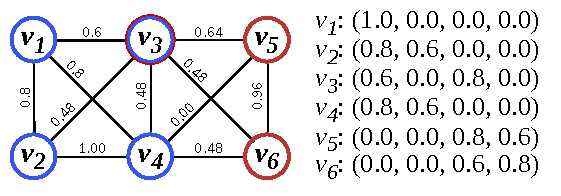
\includegraphics[width=1\linewidth,page=1]{fig/pictures.pdf}
  \caption{Example of vector-attributed graph with semantic similarities. Each vertex has a 4-dimensional vector, and edge labels show pairwise similarities.}
  \label{fig:example}
\end{figure}

\begin{example}
  \label{ex:acmsc}
  Figure~\ref{fig:example} shows a vector-attributed graph with six vertices.
  Edge labels give the precomputed pairwise similarities.
  With threshold $\tau = 0.6$, the induced subgraphs on
  $\{v_1,v_2,v_3,v_4\}$ and $\{v_3,v_4,v_5,v_6\}$ are both cliques.

  Consider the cliques:
  $C_1 = \{v_1, v_2, v_3, v_4\}$ has
  $\avgsim(C_1) = (0.80 + 0.60 + 0.80 + 0.48 + 1.00 + 0.48)/6 \approx 0.693 \geq \tau$,
  so $C_1$ is average-constrained.
  $C_2 = \{v_3, v_5, v_6\}$ has
  $\avgsim(C_2) = (0.64 + 0.48 + 0.96)/3 \approx 0.693 \geq \tau$,
  so $C_2$ is also average-constrained.
  $C_3 = \{v_3, v_4, v_5, v_6\}$ has
  $\avgsim(C_3) = (0.48 + 0.64 + 0.48 + 0.00 + 0.00 + 0.96)/6 \approx 0.427 < \tau$,
  so $C_3$ is not average-constrained despite being a valid clique.

  Moreover, no vertex can be added to $C_1$ or $C_2$ while keeping $\avgsim \geq \tau$,
  so both $C_1$ and $C_2$ are ACMSCs.
\end{example}

\stitle{Problem Statement.}
\begin{problem}[ACMSC Enumeration]
Given a vector-attributed graph $\mathcal{G}=(V,E,\mathbf{X})$ and a threshold
$\tau \in [-1,1]$, enumerate all ACMSCs of $\mathcal{G}$.
\end{problem}


\subsection{Challenges}
\label{sec:challenges}
\stitle{Hardness.}
ACMSC enumeration generalizes classical MCE: when $\tau$ is at most the
minimum pairwise similarity over all edges, every structural maximal
clique satisfies the average constraint, so ACMSC enumeration coincides
with MCE and the $\Omega(3^{n/3})$ lower bound carries over.
The associated decision problem is NP-complete.

\begin{theorem}
  \label{thm:np-complete}
Given $\mathcal{G}=(V,E,\mathbf{X})$, threshold $\tau\in[-1,1]$, and integer $k$,
  deciding whether an ACMSC of size $\geq k$ exists is \emph{NP-complete}.
\end{theorem}
\begin{proof}
  \textit{NP membership.}  A certificate is a set $C \subseteq V$.
  Verification checks: (i)~all $\binom{|C|}{2}$ pairs form edges in $O(|C|^2)$;
  (ii)~$\avgsim(C) \geq \tau$ by summing precomputed similarities in
  $O(|C|^2)$; and (iii)~for each $w \in V \setminus C$, that $C \cup \{w\}$
  is not a valid clique or violates the constraint, in $O(n \cdot |C|)$.
  All steps are polynomial in $|V|$.

  \textit{NP-hardness.}  We reduce from the \textsc{Clique} decision
  problem~\cite{karp1972}, which asks whether $G_0=(V,E)$ contains a
  clique of size $\geq k$.
  Assign $\mathbf{x}_v = \mathbf{e}_1$ to every vertex, so
  $\mathrm{sim}(u,v) = 1$ for every edge, and set $\tau = 1$.
  Under this assignment $\avgsim(C) = 1 \geq \tau$ for every clique $C$,
  so every structural maximal clique is an ACMSC and vice versa.
  Any clique of size $\geq k$ in $G_0$ is contained in some structural
  maximal clique of size $\geq k$, which is also an ACMSC of size $\geq k$.
  Conversely, any ACMSC of size $\geq k$ is a clique of size $\geq k$
  in $G_0$.  Hence a size-$k$ ACMSC exists if and only if $G_0$ contains
  a clique of size $\geq k$, completing the reduction.
\end{proof}

The output sets of ACMSC enumeration and MCE are incomparable: a structural
maximal clique with $\avgsim(M)<\tau$ may contain semantically maximal subsets
that MCE never generates, while valid ACMSCs need not be structurally maximal.
The output size, and hence the computational cost, is $\tau$-dependent in a
non-trivial way that we characterize below.

\stitle{Output Distribution and Practical Scope.}
The number of ACMSCs and their sizes vary substantially with $\tau$.
As illustrated qualitatively in Figure~\ref{fig:tau_dist}, at sufficiently
low $\tau$, almost every clique satisfies the average constraint and the
output converges toward that of classical MCE.
As $\tau$ increases, large structural cliques that previously satisfied the
constraint cease to do so and are replaced by many smaller semantically
feasible sub-cliques, none of which subsumes another.
This \emph{fragmentation effect} can inflate the output size by orders of
magnitude relative to MCE\@.
At sufficiently high $\tau$, the constraint eliminates most cliques outright
and the output shrinks considerably.

The intermediate fragmentation band carries the largest output volume and is
therefore inherently time-consuming---any correct algorithm must enumerate
all output cliques, so the output size itself imposes a lower bound on
runtime.  Low $\tau$ is appropriate when the goal is to filter out
structurally maximal cliques that are semantically too loose; high $\tau$
is appropriate when the goal is to surface only the most semantically
coherent groups.  The exact $\tau$ values at which these transitions occur
depend on the similarity distribution of the underlying dataset and cannot
be fixed a priori.

\begin{figure}[!htb]
  \centering
  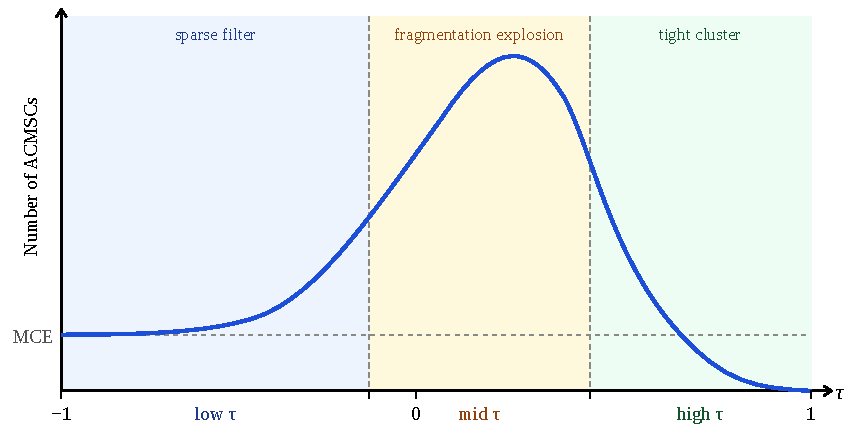
\includegraphics[width=1\linewidth]{fig/tau_distribution.pdf}
  \caption{Qualitative sketch of ACMSC count versus $\tau$.
    The dashed line marks the MCE baseline.
    The corresponding relationship between $\tau$ and intervals varies across datasets while following the same overall trend.}
  \label{fig:tau_dist}
\end{figure}

\stitle{Non-monotonicity and Framework Incompatibility.}
The core difficulty is that $\avgsim$ is non-monotone over the subset lattice.
In classical MCE, structural feasibility is monotone and maximality is enforced
implicitly by the $P=\emptyset$ invariant at every leaf, so the set of feasible
extensions can be characterized solely by the current state of $C$.
Under the average constraint, no such invariant exists: a partial clique with
$\avgsim(C)<\tau$ may still grow into a valid ACMSC, while one with
$\avgsim(C)\geq\tau$ may admit no feasible extension. Furthermore, whether a
candidate vertex can participate in a valid extension depends on its accumulated
similarity to the current partial clique, which evolves throughout the recursion
and cannot be captured by structural conditions alone. As a result, the pruning mechanisms based on structural monotonicity
lose their foundation, and the pivot strategy no longer applies.
Direct adaptations of BK are therefore forced to defer all semantic
evaluation to the leaves, where $\tau$ appears only in validation
rather than guiding the search itself.


\section{Framework}
\label{sec:framework}
\label{sec:sembk}

\stitle{Framework Overview.}
We derive a baseline search procedure by adapting the Bron--Kerbosch (BK)
recursion to the average-constrained semantic clique setting.  The standard
partition $(P,X)$ remains useful for structural enumeration, but the semantic
constraint is defined at the clique level: whether a partial clique can
eventually satisfy the threshold depends on $\avgsim$ over all vertex pairs
within the clique.  As a consequence, the pivoting strategy, which relies on
local structural properties, is no longer directly applicable.  The baseline
therefore retains the BK recursion and degeneracy ordering while excluding
pivoting, and enforces semantic maximality via a secondary \textsc{Check}
pass on $X$ at each leaf.

\begin{algorithm}[t]
  \small
  \caption{Semantic BK with Check}
  \label{alg:semantic-max-clique}
  \SetKwFunction{FSearch}{Search}
  \SetKwProg{Fn}{Function}{:}{}

  \textbf{Input}: $G=(V,E)$, semantic vectors $\{x_v\}$, threshold $\tau$\\
  \textbf{Output}: All maximal semantic cliques $C$ s.t. $\avgsim(C) \geq \tau$

  Precompute $\mathrm{sim}(u,v)$ and degeneracy ordering $\sigma$\;
  \For{each $v \in \sigma$ \textbf{in parallel}}{
    $P \leftarrow \{u \in N(v) \mid \sigma(u) > \sigma(v)\}$\;
    $X \leftarrow \{u \in N(v) \mid \sigma(u) < \sigma(v)\}$\;
    Initialize $\acc[u] \leftarrow \mathrm{sim}(u, v)$ for all $u \in N(v)$\;
    \FSearch{$C=\{v\}, \simsum=0, P, X, \acc, \textit{mode}=\emptyset, 0$}
  }

  \BlankLine
  \Fn{\FSearch{$C, \simsum, P, X, \acc, \textit{mode}, k_{\min}$}}{
    $k \leftarrow |C|,\ \textit{foundLonger} \leftarrow \mathbf{false}$\;
    \For{each $v \in P$}{
      $\simsum' \leftarrow \simsum + \acc[v]$\;
      $P \leftarrow P \setminus \{v\}, P' \leftarrow P \cap N(v), X' \leftarrow X \cap N(v)$\;
      $\acc[u] \gets \acc[u] + \mathrm{sim}(u,v)$ \textbf{for} $u \in P' \cup X'$\;
      $\textit{res} \leftarrow$ \FSearch{$C \cup \{v\}, \simsum', P', X', \acc, \textit{mode}, k_{\min}$}\;
      $\acc[u] \gets \acc[u] - \mathrm{sim}(u,v)$ \textbf{for} $u \in P' \cup X'$\;

      \If{$\textit{res}$}{
        $\textit{foundLonger} \leftarrow \mathbf{true}$\;
        \lIf{$\textit{mode} = \mathrm{CHECK}$}{\Return \textit{true}}
      }
      $X \leftarrow X \cup \{v\}$\;
    }

    \If{$\neg \textit{foundLonger}$}{
      \lIf{$k \geq 2 \land 2 \cdot \simsum / (k(k-1)) < \tau$}{\Return \textit{false}}
      \lIf{$\textit{mode} = \mathrm{CHECK}$}{\Return $k > k_{\min}$}

      \If{$X \neq \emptyset$}{
        \If{\FSearch{$C, \simsum, X, \emptyset, \acc, \mathrm{CHECK}, k$}}{
          \Return \textit{true}\;
        }
      }

      \textbf{output} $C$\;
      \Return \textit{true}\;
    }
    \Return $\textit{foundLonger}$\;
  }
\end{algorithm}

\begin{figure}[!htb]
  \centerline{\includegraphics[width=1\linewidth,page=2]{fig/pictures.pdf}}
  \caption{Search tree of Algorithm~\ref{alg:semantic-max-clique} on the example graph in Section~2.
    The traversal follows the degeneracy ordering, and each subtree corresponds to a recursive expansion in Algorithm~1.}
  \label{fig:alg1}
\end{figure}

\stitle{[Lines 4--8]: Outer Traversal.}
The outer loop iterates over vertices in degeneracy order $\sigma$.  For a
seed vertex $v$, its later neighbors under $\sigma$ form the candidate set
$P$, and its earlier neighbors are placed in $X$.  This partition guarantees
that every structural maximal clique is generated by exactly one seed,
because the unique vertex of minimum degeneracy index in any clique serves
as its seed and sees all co-members in its $P$.  Since every ACMSC is contained in at least one structural maximal clique
(as established later in Lemma~\ref{lem:containment}), the same
partition ensures completeness for the semantic problem without
modification.

\stitle{[Lines 9--29]: Recursive Search and Semantic Validation.}
Within each recursive call, the algorithm explores all vertices in $P$ as
expansion roots.  For each candidate $v$, it updates $\simsum$ and the
auxiliary accumulation array $\acc$, then recurses on the reduced candidate
and exclusion sets $(P', X')$.  When the recursion reaches a leaf
($\textit{foundLonger} = \mathbf{false}$), it first tests the average
constraint: if $\avgsim(C) < \tau$, the branch is pruned immediately.
Otherwise, semantic maximality must be verified: a clique $C$ with
$\avgsim(C) \geq \tau$ and $P = \emptyset$ could still be non-maximal if
some vertex in $X$ can extend it to a larger valid clique.  The algorithm
therefore invokes \textsc{Search} on $X$ in \textsc{Check} mode with
$k_{\min} = |C|$.  In \textsc{Check} mode, the recursion explores
extensions through $X$ and returns \textit{true} as soon as it finds any
valid clique strictly larger than $C$; if no such extension exists, $C$ is
emitted.  The strict size condition $k > k_{\min}$ is necessary because the
\textsc{Check} recursion may reach sub-cliques of $C$ itself; without
recording $k_{\min}$, these would be misidentified as valid extensions.

\stitle{Why pivoting is not used.}
In standard BK, a pivot $p \in P \cup X$ is selected so that every maximal
clique in the current branch contains either $p$ or a vertex in $P \setminus
N(p)$.  Vertices in $P \cap N(p)$ are therefore never used as expansion
roots: any maximal clique containing such a vertex $u$ must also contain $p$
and will be discovered in the sub-tree rooted at $p$.  This argument is
purely structural and relies on the fact that structural maximality is closed
under supersets.

The semantic constraint breaks this closure.  Consider $C = \emptyset$,
$P = \{p, u\}$ with $\{p,u\} \in E$, and suppose pivot $p$ is chosen so
that $u$ is suppressed as an expansion root.  The only sub-tree explored is
rooted at $p$.  If $\avgsim(\{p,u\}) < \tau$, this branch is pruned and
yields nothing.  If $\{u, w\}$ for some $w \in X$ is a valid ACMSC, it is
permanently lost: the sub-tree rooted at $u$ was never entered, and the
\textsc{Check} pass offers no remedy since it operates only on cliques
already constructed, not on suppressed sub-trees.  The absence of pivoting
is therefore a correctness requirement, not a design choice.
\stitle{Complexity.}
\begin{theorem}[Time and Space Complexity]
  \label{the:alg1complexity}
  The worst-case time complexity is $O(d \cdot n \cdot 3^{d/3})$, and the
  space complexity is $O(n + m)$, where $d$ is the degeneracy of the graph.
\end{theorem}
\begin{proof}
  The outer traversal processes each vertex once under degeneracy ordering.
  Without pivoting, the recursive procedure visits every node of the BK
  search tree, whose total size is bounded by $O(d \cdot n \cdot 3^{d/3})$
  time~\cite{eppstein2010}.  The average-threshold test costs $O(1)$
  given the maintained $\simsum$.  The \textsc{Check} recursion is invoked
  with $X$ as its candidate set and returns immediately upon finding any
  valid extension (Line~11); every node it visits is already a node in the
  BK search tree counted above, so the \textsc{Check} overhead is subsumed
  and does not alter the asymptotic bound.  Space is dominated by adjacency
  lists ($O(n+m)$) and the per-thread accumulator $\acc$ ($O(n)$);
  recursion depth is at most $O(d)$ under degeneracy ordering.
\end{proof}

\stitle{Limitations.}
While \semBK\ provides a necessary theoretical baseline for correctness, its practical utility is limited by its inability to effectively leverage pruning strategies. 
Both inefficiencies---the pivot-free branching and the
\textsc{Check} pass overhead---stem from the same root cause: the
average-similarity constraint couples all pairs inside the clique
globally and cannot be summarized through local adjacency information
alone.  As a result, the search degenerates to exhaustive structural
enumeration regardless of $\tau$, motivating the specialized algorithms
of Section~\ref{sec:algorithms}.


%%-------------------------------------------------------------------
\section{Proposed Algorithms}
\label{sec:algorithms}
This section presents two algorithms that exploit the global structure
of the average constraint from complementary directions, each targeting
a distinct region of the threshold range.

\subEnum\ (Section~\ref{sec:strsub}) resolves the pivot incompatibility
by decoupling structural and semantic search.  The pivot is applied
without modification to a $\tau$-agnostic structural phase, restoring
the $O(3^{n/3})$ BK guarantee; $\tau$ is then enforced in a subsequent
intra-clique enumeration phase. A Top-Edge Layer Pruning rule introduced in
Phase~2 skips all subset-size layers for which the sorted-edge upper
bound falls below $\tau$, giving \subEnum\ efficient performance across
the full threshold range while retaining a decisive advantage at low
$\tau$, where the structural decomposition most directly maps to the
output.

\monoSemMCE\ (Section~\ref{sec:monosem-mce}) departs from the BK
framework entirely.  Motivated by the observation that \subEnum, despite
its pruning improvements, still processes all structural maximal cliques
irrespective of their semantic quality, \monoSemMCE\ introduces a
monotone-path search strategy in which $\tau$ drives the enumeration
from the first expansion step.  The resulting feasibility window enables
suffix-level pruning in $O(1)$, making \monoSemMCE\ particularly
efficient in the high-$\tau$ regime where semantically coherent groups
are rare and the window is narrow.

Together, the two algorithms constitute the main contributions of this
paper.  \subEnum\ is efficient across the full threshold range, with
its strongest advantage at low $\tau$; \monoSemMCE\ delivers superior
high-$\tau$ efficiency through a fundamentally different algorithmic
paradigm.  Their complementary strengths cover the practically
meaningful operating ranges identified in Section~\ref{sec:challenges}.

%%-------------------------------------------------------------------
\subsection{\subEnum: Structural Decomposition and Subset Enumeration}
\label{sec:strsub}

\stitle{Structural--Semantic Decoupling and Containment.}
The validity of the Bron--Kerbosch pivot rests on a structural invariant:
every structural maximal clique must contain at least one vertex from
$P \setminus N(u)$ for any pivot $u \in P \cup X$.  This invariant is
violated when the average-similarity constraint is incorporated directly
into the branching procedure, because $\avgsim$ is a \emph{global}
property of a candidate set and does not decompose along the local
neighborhood structure used to justify the pivot.  Consequently, the
semantic variant \semBK\ must forgo pivoting entirely, which
undermines the $O(3^{n/3})$ worst-case guarantee of the standard
algorithm~\cite{tomita2006worst}.

\begin{algorithm}[t]
  \small
  \caption{\subEnum: Structural Decomposition and Subset Enumeration}
  \label{alg:strsub}
  \SetKwFunction{FBK}{BK}
  \SetKwProg{Fn}{Function}{:}{}

  \KwIn{$G=(V,E)$, similarities $\{\mathrm{sim}(u,v)\}_{(u,v)\in E}$, threshold $\tau$}
  \KwOut{All ACMSCs $\mathcal{R}$}

  \tcc{Phase 1: Structural MCE}
  Build degeneracy ordering $\sigma$\;
  $\mathcal{M} \leftarrow \emptyset$\;
  \For{each $v \in \sigma$ \textbf{in parallel}}{
    $P \leftarrow \{u \in N(v) \mid \sigma(u) > \sigma(v)\}$\;
    $X \leftarrow \{u \in N(v) \mid \sigma(u) < \sigma(v)\}$\;
    $\mathcal{M} \leftarrow \mathcal{M} \cup \FBK{\{v\},\ P,\ X}$\;
  }

  \tcc{Phase 2: Intra-clique semantic enumeration}
  $\mathcal{F} \leftarrow \emptyset$\;
  \For{each $M \in \mathcal{M}$ \textbf{in parallel}}{
    \lIf{$\avgsim(M) \geq \tau$}{$\mathcal{F} \leftarrow \mathcal{F} \cup \{M\}$; \textbf{continue}}
    \tcc{Top-Edge Layer Pruning: skip sizes whose best-case mean falls below $\tau$}
    Sort edges of $M$ by similarity descending\;
    $k^* \leftarrow \max\!\bigl\{k \in [2,|M|-1] \mid \bar{e}_k \geq \tau\bigr\}$\;
    \lIf{$k^*$ does not exist}{\textbf{continue}}
    $\mathit{lmax} \leftarrow \emptyset$;\quad $\mathit{umask} \leftarrow \mathbf{0}$\;
    \For{$k \leftarrow k^*$ \KwTo $2$}{
      \For{each size-$k$ subset $S \subseteq M$}{
        \lIf{$(S \mathbin{\&}\ \mathit{umask}) = S$
          \textbf{ and } $\exists\, T \in \mathit{lmax} : S \subseteq T$}{\textbf{continue}}
        \If{$\avgsim(S) \geq \tau$}{
          $\mathit{lmax} \leftarrow \mathit{lmax} \cup \{S\}$\;
          $\mathit{umask} \leftarrow \mathit{umask} \mid S$\;
          $\mathcal{F} \leftarrow \mathcal{F} \cup \{S\}$\;
        }
      }
    }
  }

  \tcc{Phase 3: Global deduplication}
  Sort $\mathcal{F}$ by $|\cdot|$ descending; remove exact duplicates\;
  Build inverted index $\mathit{inv}: v \mapsto \{S \in \mathcal{F} \mid v \in S\}$\;
  $\mathcal{R} \leftarrow \emptyset$\;
  \For{each $S \in \mathcal{F}$ in order}{
    $r \leftarrow \displaystyle\mathop{\arg\min}_{v \in S}\ |\mathit{inv}[v]|$\;
    \lIf{$\exists\, T \in \mathcal{R}$ via $\mathit{inv}[r]$ s.t.\ $S \subsetneq T$}{\textbf{continue}}
    $\mathcal{R} \leftarrow \mathcal{R} \cup \{S\}$\;
  }
  \Return $\mathcal{R}$\;
\end{algorithm}
\begin{figure}[!htb]
  \centerline{\includegraphics[width=1\linewidth,page=3]{fig/pictures.pdf}}
  \caption{Complete three-phase execution of Algorithm~\ref{alg:strsub} on the example graph in Section~2.
    Phase~1 shows the BK search tree under degeneracy ordering, producing all structural maximal cliques.
    Phase~2 illustrates intra-clique subset enumeration with the local maximality filter applied within each clique.
    Phase~3 depicts global deduplication via the inverted index, retaining only non-subsumed ACMSCs.}
  \label{fig:alg2}
\end{figure}


The key insight behind \subEnum\ is that the structural and semantic
layers of the problem can be \emph{decoupled}.  Specifically, the
Tomita pivot can be applied without modification to the purely
structural problem of enumerating maximal cliques in $G$, because that
problem carries no average-similarity constraint.  The threshold $\tau$
is then enforced in a second, independent pass confined to each
structural maximal clique.  The theoretical basis for this decoupling
is the following containment lemma.

\begin{lemma}[Structural Superset of ACMSCs]
  \label{lem:containment}
  Every ACMSC is contained in at least one structural maximal clique of $G$.
  That is, for every ACMSC $C$, there exists a structural maximal clique
  $M$ such that $C \subseteq M$.
\end{lemma}

\begin{proof}
  By definition, every ACMSC is a clique of $G$.  Let $C$ be an arbitrary
  ACMSC, and consider the family
  \[
    \mathcal{F} = \{D \subseteq V \mid C \subseteq D \text{ and } D
    \text{ is a clique in } G\}.
  \]
  Since $C \in \mathcal{F}$, the family is nonempty.  Because $V$ is
  finite, $\mathcal{F}$ is finite, so we may choose a set $M \in
    \mathcal{F}$ that is maximal under inclusion.  By construction, $M$ is
  a clique containing $C$, and no vertex $w \in V \setminus M$ extends $M$
  to a larger clique; hence $M$ is a structural maximal clique of $G$,
  and $C \subseteq M$.
\end{proof}

Lemma~\ref{lem:containment} establishes that the complete collection of
ACMSCs can be recovered by (i)~enumerating all structural maximal
cliques, and (ii)~searching within each structural maximal clique for
semantically feasible maximal subsets.  Step~(i) is a purely structural
problem to which the full Tomita pivot applies, restoring the
$O(3^{n/3})$ worst-case bound of standard BK\@.  The threshold $\tau$
enters only in step~(ii), where the search space is bounded by the size
of a single structural clique.  Algorithm~\ref{alg:strsub} implements
this strategy in three phases.

\stitle{[Lines 1--6]: Phase~1 -- Structural Maximal Clique Enumeration.}
Phase~1 enumerates all structural maximal cliques of $G$ using the
standard BK algorithm equipped with the Tomita pivot~\cite{tomita2006worst}
and degeneracy ordering~\cite{eppstein2013listing}.  Vertices are
processed in degeneracy order $\sigma$; for each seed vertex $v$, the
candidate set $P$ and exclusion set $X$ are initialized to the
forward and backward neighborhoods of $v$ in $\sigma$, respectively,
and recursive BK is invoked on the triple $(\{v\}, P, X)$.  Seeds are
dispatched in parallel via OpenMP dynamic scheduling.  Crucially, this
phase is entirely $\tau$-agnostic: the threshold plays no role in
branching decisions, so the full pivot strategy and its associated
complexity bound are preserved.

\stitle{[Lines 7--20]: Phase~2 -- Intra-Clique Semantic Enumeration.}
For each structural maximal clique $M$ of size $m$ produced by Phase~1,
Phase~2 enumerates all semantically maximal subsets of $M$ with respect
to $\tau$.  Subsets of $M$ are generated in descending order of
cardinality using bitmask iteration (Gosper's hack), and pairwise
similarities are precomputed into an $m \times m$ local matrix to amortize
repeated $\avgsim$ evaluations.

A \emph{local maximality filter} prunes redundant candidates during
enumeration.  The filter maintains a set $\mathit{lmax}$ of valid
subsets discovered so far within $M$, together with a union mask
$\mathit{umask} = \bigcup_{T \in \mathit{lmax}} T$ that provides a
constant-time necessary condition for subsumption.  A candidate subset
$S$ is skipped if $S \subseteq T$ for some $T \in \mathit{lmax}$,
verified first via the bitmask test $(S \mathbin{\&}\ \mathit{umask}) = S$
and then by a linear scan over $\mathit{lmax}$.  This filter is correct
because, if $S \subsetneq T$ and $\avgsim(T) \geq \tau$, then $S$
cannot be semantically maximal in $G$ regardless of its own average
similarity.  Cliques in $\mathcal{M}$ are processed in parallel. The enumeration starting size is further reduced by Top-Edge Layer
Pruning, described below.

\stitle{[Lines 21--28]: Phase~3 -- Global Deduplication.}
Because the same ACMSC may be structurally contained in multiple
distinct maximal cliques, Phase~2 may emit duplicate or subsumed
candidates across cliques.  Phase~3 consolidates these candidates into
the final result set $\mathcal{R}$.

The phase proceeds in two steps.  First, all candidates in $\mathcal{F}$
are sorted lexicographically and exact duplicates are removed in
$O(N \log N)$ time, where $N = |\mathcal{F}|$.  Second, subsumption is
detected via an inverted index $\mathit{inv}: v \mapsto \{S \in
  \mathcal{F} \mid v \in S\}$.  For each candidate $S$, the algorithm
identifies its \emph{rarest vertex} $r = \arg\min_{v \in S}
  |\mathit{inv}[v]|$ and scans only the list $\mathit{inv}[r]$; a
sorted-merge traversal then determines in $O(|S| + |T|)$ time whether
$S \subsetneq T$ for some already-accepted candidate $T \in
  \mathcal{R}$.  If no such $T$ exists, $S$ is added to $\mathcal{R}$.


\stitle{Top-Edge Layer Pruning.}
Phase~2 as described iterates over all subset sizes from $|M|-1$ down
to $2$.  A key observation allows the starting size to be reduced: the
best achievable $\avgsim$ for any size-$k$ subset of $M$ is bounded
above by the mean of the $\binom{k}{2}$ largest pairwise similarities
in $M$.

\begin{property}[Sorted-Edge Upper Bound]
\label{prop:topk}
Let $e_1 \geq e_2 \geq \cdots \geq e_{\binom{m}{2}}$ be the pairwise
similarities of $M$ sorted in descending order.  For any size-$k$
subset $S \subseteq M$,
\[
  \avgsim(S) \;\leq\; \bar{e}_k
  \;:=\; \frac{1}{\tbinom{k}{2}} \sum_{i=1}^{\tbinom{k}{2}} e_i.
\]
\end{property}

\begin{proof}
Any size-$k$ subset $S \subseteq M$ uses exactly $\binom{k}{2}$ pairs,
each contributing at most the corresponding value in the sorted sequence
$e_1 \geq e_2 \geq \cdots$; hence $\simsum(S) \leq \sum_{i=1}^{\binom{k}{2}} e_i$,
and dividing both sides by $\binom{k}{2}$ gives the result.
\end{proof}
Note that $\bar{e}_k$ is non-increasing in $k$: a larger subset requires
more edges, drawing further into the sorted list and lowering the mean.
Before enumeration, all pairwise similarities of $M$ are sorted once in
$O(m^2 \log m)$ and prefix means $\bar{e}_k$ are computed for all $k$.
The algorithm identifies
\[
  k^* = \max\!\bigl\{k \in [2, |M|-1] \;\big|\; \bar{e}_k \geq \tau\bigr\},
\]
and begins enumeration at $k = k^*$ rather than $|M|-1$.  Because
$\bar{e}_k$ is non-increasing, all sizes $k > k^*$ satisfy
$\bar{e}_k < \tau$, certifying that no subset of those sizes can meet
the constraint; they are skipped entirely.  If no such $k^*$ exists,
the whole clique $M$ is skipped.  This layer pruning is reflected in
Lines~8--10 of Algorithm~\ref{alg:strsub}.

\stitle{Characteristics and Applicable Regime.}
\subEnum\ inherits the full efficiency of BK with Tomita pivot in
Phase~1, which runs in $O(dn \cdot 3^{d/3})$ time independently of
$\tau$.  At low $\tau$, nearly every subset of a structural maximal
clique satisfies the average constraint, so the local maximality filter
rapidly identifies large valid subsets and terminates Phase~2 early.
The Top-Edge Layer Pruning extends this efficiency to medium and high
$\tau$: for most structural cliques $M$, either the whole clique is
accepted immediately ($\avgsim(M) \geq \tau$) or $k^*$ is small,
confining bitmask enumeration to a narrow band of sizes near the base.
In the extreme high-$\tau$ regime, however, \subEnum\ still processes
every structural maximal clique in Phase~1 regardless of semantic
quality; when most structural cliques are semantically barren, this
overhead becomes the bottleneck.  \monoSemMCE\ addresses this by
integrating $\tau$ into the search from the outset, never generating
semantically infeasible states.

\stitle{Complexity.}
\begin{theorem}[Time Complexity of \subEnum]
  \label{the:alg2complexity}
  \subEnum\ runs in
  $O\!\left(dn \cdot 3^{d/3} + \sum_{M \in \mathcal{M}} 2^{|M|} \cdot |M|^2
    + N \log N + \sum_{S \in \mathcal{F}} L_{\min}(S)\right)$
  time, where $d$ is the degeneracy of $G$, $N = |\mathcal{F}|$ is the
  number of candidates before deduplication, and $L_{\min}(S) =
  \min_{v \in S}|\mathit{inv}[v]|$.
\end{theorem}
\begin{proof}
  \textbf{Phase~1.}  With degeneracy ordering, BK with Tomita pivot runs
  in $O(dn \cdot 3^{d/3})$ time~\cite{eppstein2013listing}.

  \textbf{Phase~2.}  For a structural maximal clique $M$ of size $m$,
  bitmask enumeration visits at most $2^m$ subsets.  Each subset $S$
  requires computing $\avgsim(S)$ from the precomputed $m \times m$
  similarity matrix at cost $O(|S|^2) \leq O(m^2)$.  The per-clique
  cost is therefore $O(2^m \cdot m^2)$, giving
  $\sum_{M \in \mathcal{M}} O(2^{|M|} \cdot |M|^2)$ overall.
  The union-mask pre-filter and local maximality scan do not increase
  this asymptotic bound.

  \textbf{Phase~3.}  Lexicographic sorting costs $O(N \log N)$.  For
  each candidate $S$, the algorithm scans $\mathit{inv}[r]$ of length
  $L_{\min}(S)$; each of the at most $L_{\min}(S)$ subsumption checks
  costs $O(|S| + |T|)$ via sorted-merge comparison, where $|S|$ and
  $|T|$ are at most $\bar{k}$ (the average candidate size, a problem
  parameter).  Treating $\bar{k}$ as a constant, the total Phase~3
  cost is $O\!\left(N \log N + \sum_{S \in \mathcal{F}} L_{\min}(S)\right)$.
\end{proof}

\noindent\textbf{Remark.}
The $\sum_{M \in \mathcal{M}} 2^{|M|} \cdot |M|^2$ term is a worst-case
bound on Phase~2 without pruning.  In practice, Top-Edge Layer Pruning
(Property~\ref{prop:topk}) restricts enumeration to sizes $k \leq k^*$,
reducing the per-clique cost to
$O\!\left(|M|^2 \cdot \sum_{k=2}^{k^*} \binom{|M|}{k}\right)$,
which is substantially smaller than $2^{|M|} \cdot |M|^2$ whenever
$k^*$ is small relative to $|M|$.


%%-------------------------------------------------------------------
\subsection{\monoSemMCE: Live Enumeration with Monotone-Path Constraint}
\label{sec:monosem-mce}

\stitle{Motivation and Core Insight.}
Even with the Top-Edge Layer Pruning, \subEnum\ is bound to Phase~1: it enumerates
all structural maximal cliques before any semantic evaluation takes
place.  In the high-$\tau$ regime, the vast majority of structural
cliques may be semantically barren, yet each still contributes Phase~1
cost.  More fundamentally, the BK framework offers no mechanism to
incorporate $\tau$ into branching decisions---the threshold appears only
in validation, never in the search logic itself.  This structural
overhead motivates abandoning the BK skeleton entirely.

The obstacle to integrating $\tau$ directly into search is the
non-monotonicity of $\avgsim$ over the subset lattice: adding a vertex
may raise or lower the average, so infeasibility at depth $d$ carries
no implication for depth $d{+}1$.  This precludes any branch-and-bound
strategy based on the current average alone.

We resolve this with a single structural observation
(Theorem~\ref{thm:monotone}): \emph{every ACMSC admits a vertex
insertion ordering along which $\avgsim$ is non-increasing at every
step}.  This monotone path property imposes a global ordering structure
on an apparently unordered combinatorial object.  Restricting the search
to monotone paths is complete by the theorem, and induces a
\emph{sorted-suffix cut} that discards an entire ordered suffix of
candidates in $O(1)$---qualitatively stronger than any per-candidate
\textbf{continue} in prior work.  A complementary lower-end cut
($W$-pruning) eliminates infeasible candidates from the opposite end.
Together they define a \emph{feasibility window} over sorted candidates
that contracts rapidly as $\tau$ increases.

These insights motivate a clean BK-free architecture.  \monoSemMCE\
replaces recursive BK with \emph{level-synchronous} expansion: layer
$\ell$ holds all live $(\ell{+}2)$-cliques satisfying $\avgsim \geq
\tau$, each expanded in parallel to produce layer $\ell{+}1$.  Every
clique in every layer is semantically live by construction---no
structurally valid but semantically infeasible state is ever generated
or stored.  This makes \monoSemMCE\ the algorithm of choice for
high-$\tau$ ACMSC enumeration, where the feasibility window is narrow
and the pruning is most aggressive.

\stitle{The Monotone Path Property.}

\begin{theorem}[Monotone Path Property]
  \label{thm:monotone}
  Let $S = \{v_1, \ldots, v_k\}$ be an ACMSC with $k \geq 2$.  There
  exists a permutation $\pi$ of $\{1,\ldots,k\}$ such that
  \[
    \avgsim\!\bigl(\{v_{\pi(1)}, \ldots, v_{\pi(i)}\}\bigr)
    \;\geq\;
    \avgsim\!\bigl(\{v_{\pi(1)}, \ldots, v_{\pi(i+1)}\}\bigr)
  \]
  for every $i \in \{1, \ldots, k-1\}$.
\end{theorem}

\begin{proof}[Proof sketch]
  We construct $\pi$ by a greedy removal argument.  Define the marginal
  contribution of $v \in S$ as $\delta_v = \acc[v]$, the total similarity
  of $v$ to the remaining nodes.  We claim some $v^* \in S$ satisfies
  $\avgsim(S \setminus \{v^*\}) \geq \avgsim(S)$.  Suppose for
  contradiction that every $v \in S$ raises the average upon removal.
  Summing the identity
  $k(k{-}1)\avgsim(S) = (k{-}1)(k{-}2)\avgsim(S\setminus\{v\}) +
    2\delta_v$ over all $v \in S$ and using
  $\sum_v \delta_v = 2\,\simsum(S)$ yields
  $k \cdot \avgsim(S) < k \cdot \avgsim(S)$, a contradiction.  Greedy
  removal of the minimum-contribution vertex at each step produces a
  sequence whose reversal is the required non-increasing insertion
  ordering $\pi$.  The full inductive argument is deferred to
  Appendix~\ref{app:monotone}.
\end{proof}

\begin{figure}[t]
  \centering
  \includegraphics[width=0.9\linewidth,page=5]{fig/pictures.pdf}
  \caption{A monotone expansion path: the average similarity decreases from 1.00 (2-clique) to 0.86 (3-clique) to 0.69 (4-clique).}
  \label{fig:monotone}
\end{figure}

\begin{algorithm}[t]
  \small
  \caption{\monoSemMCE: Level-Synchronous Clique Expansion}
  \label{alg:monosem-mce}
  \SetKwFunction{FExpand}{Expand}
  \SetKwProg{Fn}{Function}{:}{}
  \textbf{Input}: $G=(V,E)$, semantic vectors $\{x_v\}$, threshold $\tau$\\
  \textbf{Output}: All ACMSCs $\mathcal{R}$

  Precompute $\mathrm{sim}(u,v)$ for all $(u,v)\in E$\;
  $\mathcal{F} \leftarrow \emptyset$\;
  \tcc{Layer 0: seed all valid edges as 2-cliques}
  $\mathcal{L}_0 \leftarrow \bigl\{\,(C,\simsum,P,\acc)\bigr\}$ for each $(u,v)\in E$ with $\mathrm{sim}(u,v)\geq\tau$,
  where $C\!=\!\{u,v\}$, $\simsum\!=\!\mathrm{sim}(u,v)$,
  $P\!=\!N(u)\cap N(v)$,
  $\acc[w]\!=\!\mathrm{sim}(w,u)+\mathrm{sim}(w,v)\ \forall w\!\in\! P$\;
  Deduplicate $\mathcal{L}_0$ by $C$\;
  $\ell \leftarrow 0$\;
  \While{$\mathcal{L}_\ell \neq \emptyset$}{
    $\mathcal{L}_{\ell+1} \leftarrow \emptyset$\;
    \For{each $(C,\simsum,P,\acc) \in \mathcal{L}_\ell$ \textbf{in parallel}}{
      \FExpand{$C,\ \simsum,\ P,\ \acc,\ \mathcal{L}_{\ell+1},\ \mathcal{F}$}\;
    }
    Deduplicate $\mathcal{L}_{\ell+1}$ by $C$\;
    $\ell \leftarrow \ell + 1$\;
  }
  \Return $\mathcal{R} \leftarrow \mathcal{F}$\;
  \BlankLine
  \Fn{\FExpand{$C,\ \simsum,\ P,\ \acc,\ \mathcal{L}_{\text{next}},\ \mathcal{F}$}}{
  $k \leftarrow |C|$,\quad $\W \leftarrow \simsum - \tau\tbinom{k}{2}$\;
  Sort $P$ by $\acc[\cdot]$ ascending\;
  $\textit{has\_valid} \leftarrow \textbf{false}$\;
  $\textit{any\_extended} \leftarrow \textbf{false}$\;
  \For{each $v \in P$}{
  $\delta_v \leftarrow \acc[v]$\;
  \tcc{$W$-prune}
  \lIf{$\W + \delta_v < \tau \cdot k$}{\textbf{continue}}
  $\textit{has\_valid} \leftarrow \textbf{true}$\;
  \tcc{monotone break}
  \lIf{$k \geq 2$ \textbf{ and } $\delta_v > \avgsim(C)\cdot\tbinom{k+1}{2} - \simsum$}{\textbf{break}}
  $P' \leftarrow P \cap N(v)$\;
  $\acc'[w] \leftarrow \acc[w] + \mathrm{sim}(w,v)$ for all $w \in P'$\;
  Sort $P'$ by $\acc'[\cdot]$ ascending\;
  Add $\bigl(C\cup\{v\},\ \simsum+\delta_v,\ P',\ \acc'\bigr)$ to $\mathcal{L}_{\text{next}}$\;
  $\textit{any\_extended} \leftarrow \textbf{true}$\;
  }
  \lIf{\textbf{not} $\textit{any\_extended}$ \textbf{ and not} $\textit{has\_valid}$ \textbf{ and } $k \geq 2$ \textbf{ and } $\W \geq 0$}{$\mathcal{F} \leftarrow \mathcal{F} \cup \{C\}$}
  }
\end{algorithm}
\begin{figure}[!htb]
  \centerline{\includegraphics[width=1\linewidth,page=4]{fig/pictures.pdf}}
  \caption{Execution of Algorithm~\ref{alg:monosem-mce} on the example
    graph from Section~2.  Each row corresponds to one layer
    $\mathcal{L}_\ell$, containing all live $(\ell{+}2)$-cliques with
    $\avgsim \geq \tau$. }
  \label{fig:alg3}
\end{figure}

\stitle{[Lines 3--7]: Layer Initialization.}
The algorithm seeds $\mathcal{L}_0$ with every edge $(u,v)$ satisfying
$\mathrm{sim}(u,v) \geq \tau$, representing all valid 2-cliques.  Each
state carries the clique $C$, the accumulated similarity sum $\simsum$,
the common-neighbor candidate set $P$, and the per-candidate accumulated
similarity vector $\acc$.  This initialization constitutes a fundamental
departure from BK: there is no global exclusion set $X$ and no seed
ordering constraint.  Any valid 2-clique is a legitimate root, and
correctness is guaranteed not by the BK ordering invariant but by
per-layer deduplication---a design that decouples enumeration
correctness from vertex ordering entirely.

\stitle{[Lines 8--13]: Level-Synchronous Expansion.}
The outer loop advances layer by layer.  All states in $\mathcal{L}_\ell$
are expanded in parallel to produce $\mathcal{L}_{\ell+1}$, which is
deduplicated before the next iteration.  Because every state satisfies
$\avgsim \geq \tau$ by construction, the search operates entirely within
the semantically feasible region: unlike BK-based approaches, no
structurally valid but semantically infeasible state is ever generated
or stored.

\stitle{[Lines 15--30]: Pruning Within \textsc{Expand}.}
Both pruning rules operate on the candidate list sorted by $\delta_v$
ascending.

\smallskip
\noindent\textbf{$W$-pruning (Lines~22--23).}
Define the semantic surplus $\W(C) = \simsum - \tau\binom{k}{2}$, so
that $\W \geq 0$ iff $\avgsim(C) \geq \tau$.  Adding $v$ yields
$\W(C \cup \{v\}) = \W + \delta_v - \tau k$.  If this is negative,
$v$ is skipped (\textbf{continue}); because the list is sorted
ascending, this eliminates the entire low-$\delta_v$ prefix.

\smallskip
\noindent\textbf{Monotone break (Line 24).}
Adding $v$ lowers $\avgsim$ iff $\delta_v \leq \avgsim(C) \cdot
  \binom{k+1}{2} - \simsum =: \dlim$.  The first candidate with
$\delta_v > \dlim$ would raise $\avgsim$, violating the monotone-path
invariant; by Theorem~\ref{thm:monotone}, no ACMSC is reachable through
any such candidate.  Because the list is sorted, all subsequent
candidates also exceed $\dlim$, so the entire remaining suffix is
discarded with a single \textbf{break}.  This is the key advance: one
comparison eliminates an ordered suffix of arbitrary length in $O(1)$.

Together, the two rules define a feasibility window
$[\delta_{\mathrm{lo}}, \dlim]$; only candidates within this window
are expanded.  As $\tau$ increases, both boundaries tighten
simultaneously and the window narrows rapidly, making \monoSemMCE\
effectively output-sensitive in the high-$\tau$ regime.

\stitle{Global Deduplication.}
Per-layer deduplication suppresses redundant expansion of identical
clique states within each layer.  However, the emission condition
certifies local maximality only along a single monotone path: a clique
$C$ that cannot be extended via any monotone-compatible candidate in its
current sub-tree may still be a proper subset of a larger ACMSC
reachable from a different root via a different path.  Such cross-path
subsumption is invisible during expansion and must be detected
post-hoc.  A final global deduplication pass (using the inverted-index procedure
of Phase~3 of \subEnum) removes all subsumed candidates.  By
Theorem~\ref{thm:monotone}, every ACMSC $C^*$ is reachable via its
non-increasing insertion ordering: each prefix satisfies $\avgsim \geq
\tau$, so neither pruning rule discards it, and $C^*$ is eventually
emitted; deduplication then retains $C^*$ if and only if no larger
ACMSC contains it, yielding the correct output $\mathcal{R}$.


\stitle{Complexity.}
\begin{theorem}[Time and Space Complexity of \monoSemMCE]
  \label{thm:monosem-complexity}
  Let $F$ denote the total number of clique states processed across all
  layers, $\Delta$ the maximum degree of $G$, $N = |\mathcal{F}|$ the
  number of emitted candidates before global deduplication, $L_{\min}(S)
  = \min_{v \in S}|\mathit{inv}[v]|$ the rarest-vertex inverted list
  length for candidate $S$, and $\bar{k}$ the average candidate clique
  size.  \monoSemMCE\ runs in
  \[
    O\!\left(F \cdot \Delta \log \Delta \;+\; N \log N \;+\;
    \sum_{S \in \mathcal{F}} L_{\min}(S)\right)
  \]
  time and uses $O\!\left(F \cdot \Delta + N \cdot \bar{k}\right)$ space.
\end{theorem}

\begin{proof}
  \textbf{Expansion.}
  Each \textsc{Expand} call sorts $P$ in $O(\Delta \log \Delta)$ and
  produces $w_i \geq 0$ child states.  Each child state requires a
  neighbor intersection and $\acc$ update in $O(\Delta)$, followed by
  sorting the child candidate list in $O(\Delta \log \Delta)$; the cost
  per child is thus $O(\Delta \log \Delta)$.  The total cost of a single
  call is $O((1 + w_i)\Delta \log \Delta)$.  Summing over all $F$
  processed states and using $\sum_i w_i \leq F$ (since each child state
  is itself counted in $F$) gives $O(F \cdot \Delta \log \Delta)$.

  \textbf{Per-layer deduplication.}
  Lexicographic sorting within layer $\ell$ costs $O(F_\ell \cdot \ell
  \log F_\ell)$.  Since layer $\ell$ contains $(\ell{+}2)$-cliques and
  clique size is at most $\Delta + 1$, we have $\ell \leq \Delta - 1$.
  Summing over all layers: $\sum_\ell F_\ell \cdot \ell \log F_\ell
  \leq \Delta \log F \cdot \sum_\ell F_\ell = O(F \cdot \Delta \log F)$,
  which is $O(F \cdot \Delta \log \Delta)$ when $F \leq \Delta^{O(1)}$
  and at most an additive $O(F \cdot \Delta \log F)$ otherwise.

  \textbf{Global deduplication.}
  Sorting $N$ candidates costs $O(N \log N)$.  For each $S$, the
  rarest-vertex scan examines at most $L_{\min}(S)$ candidates from
  $\mathit{inv}[r]$; each subsumption check costs $O(|S| + |T|) \leq
  O(\bar{k})$.  Treating $\bar{k}$ as a constant, the total cost is
  $O\!\left(N \log N + \sum_{S \in \mathcal{F}} L_{\min}(S)\right)$.

  \textbf{Space.}
  At most two consecutive layers are held in memory simultaneously;
  each state occupies $O(\Delta)$ words, giving $O(F \cdot \Delta)$
  for the working memory.  The candidate set $\mathcal{F}$ requires
  $O(N \cdot \bar{k})$ additional space.
\end{proof}

\noindent\textbf{Remark.}
$F$ is governed by the width of the feasibility window
$[\delta_{\mathrm{lo}}, \dlim]$ at each expansion node.  In the
high-$\tau$ regime, both pruning boundaries tighten simultaneously,
$F$ approaches the number of ACMSCs multiplied by a small depth factor,
and \monoSemMCE\ is effectively output-sensitive.  As $\tau$ decreases,
the window widens and the number of live states $F$ grows; in the
low-$\tau$ regime, \subEnum\ is the more appropriate choice, as its
structural decomposition remains efficient precisely where the
monotone-path window offers little pruning power.

\section{Implementation Optimizations}
\label{sec:opt}

The following optimizations are applied to \monoSemMCE\ and \subEnum\
without affecting correctness.  They address three categories of
bottlenecks: parallel load balance, repeated computation in the
expansion inner loop, and memory access cost for neighbor intersection
and similarity lookup.

\stitle{Level-Synchronous Parallelism and Load Balance.}
\subEnum\ Phase~1 parallelizes BK over seed vertices under degeneracy
ordering: each seed $v$ spawns an independent subproblem over its
forward neighborhood $(P_v, X_v)$, and distinct seeds share no mutable
state and require no synchronization.  Phase~2 processes each
structural maximal clique independently with thread-local candidate
lists merged once after completion, avoiding lock contention on the
output.  The decomposition is coarse-grained: each work unit is a full
BK subtree rooted at a seed, whose cost is unknown until completion and
varies substantially across seeds.

\monoSemMCE\ decomposes at finer granularity: each work unit is a
single \textsc{Expand} call on one clique state, costing $O(|P| \log
  |P|)$ where $|P|$ is the candidate set size of that state.  All states
in $\mathcal{L}_\ell$ are dispatched independently under dynamic
scheduling with no inter-state dependencies, so the scheduler can
continuously rebalance work across threads.  The cost of this design
is a synchronization barrier between layers: deduplicating
$\mathcal{L}_{\ell+1}$ requires a global sort costing
$O(|\mathcal{L}_{\ell+1}| \log |\mathcal{L}_{\ell+1}|)$ before the
next layer begins.  This is the only serialization point in
\monoSemMCE.

\stitle{Incremental Candidate Maintenance.}
When expanding state $(C, \simsum, P, \acc)$ by vertex $v$, the child
state requires an updated candidate set $P' = P \cap N(v)$ and an
updated accumulator $\acc'$.  A na\"{i}ve implementation recomputes
$\acc'$ from scratch at cost $O(|P'| \cdot |C|)$ per expansion.

Since $\acc[w] = \sum_{u \in C} \mathrm{sim}(w, u)$, the child
accumulator satisfies
\[
  \acc'[w] = \acc[w] + \mathrm{sim}(w, v) \quad \forall\, w \in P',
\]
reducing the update to $O(|P'|)$ regardless of clique depth.
Filtering $P$ to $N(v)$ preserves the relative order of retained
entries under $\acc[\cdot]$; the scalar increment $\mathrm{sim}(w,v)$
is then applied to each entry before a final sort.  The sort cost is
$O(|P'| \log |P'|)$.

\stitle{Sparse Blocked Bitmap for Neighbor Intersection.}
Candidate set intersection $P' = P \cap N(v)$ is the innermost
operation of every expansion.  We represent each adjacency list as a
\emph{sparse blocked bitmap}: vertices are indexed by
$\lfloor v/64 \rfloor$, and only non-empty 64-bit blocks are stored as
(index, word) pairs in sorted order.  Intersection of two rows
executes a merge-style scan over their block lists, applying bitwise
AND only to matching block indices and extracting set bits via
\texttt{ctz}.  The cost is $O(b_u + b_v)$ where $b_u, b_v$ count
non-empty blocks in each row, compared to $O(n/64)$ for a dense
bitmap.

This advantage compounds with search depth: at layer $\ell$, every
candidate $w \in P$ is a common neighbor of all $\ell{+}2$ clique
members, so $|P|$ decreases with $\ell$ and each row's active block
count shrinks accordingly.  The per-intersection cost therefore
decreases with depth.

\stitle{Similarity Computation with Reorder-Aware Caching.}
All pairwise similarities are precomputed once and stored in sorted
adjacency lists for $O(\log \deg(u))$ lookup via binary search.
Inner products use AVX2 8-wide SIMD, processing 8 float
multiplications per cycle.

To reduce cache miss cost on repeated lookups, vertices are reordered
by a degree-descending BFS before vectors are stored contiguously in
memory.  A vertex $u$ with degree $d_u$ participates in $O(d_u)$
expansions as a candidate across the search; placing high-degree
vertices at low memory offsets concentrates the most frequently
accessed vectors into a small number of cache lines, reducing cold
misses on the hot working set.
\section{Experiments}
\label{sec:exp}

\subsection{Experimental Setup}
\label{sec:exp-setup}

\stitle{Algorithms.}
We evaluate five algorithms.
\textbf{\StructBK} is a high-performance maximal clique enumeration
baseline that integrates degeneracy ordering to reduce candidate set
size, pivot-based pruning as in the Tomita algorithm to limit
branching, bitmap-based set representations to accelerate intersection
operations, and multi-threaded parallelization for efficiency.
It does not target the same problem as our method, since it enumerates
all maximal cliques without considering semantic constraints.
Instead, it serves as a structural upper bound on the search complexity
in the absence of attribute filtering, providing a reference for
understanding the reduction in search space achieved by our approach.
\textbf{\baseline} is a placeholder for a second baseline method.
\textbf{\semBK}, \textbf{\subEnum}, and \textbf{\monoSemMCE}
are our proposed algorithms described in
Sections~\ref{sec:sembk}--\ref{sec:monosem-mce}.

\stitle{Datasets.}
We use ten real-world graphs summarized in Table~\ref{tab:datasets}.
Datasets~1--6 are structural graphs; datasets~7--10 carry natural
language entity descriptions.  For structural graphs, each vertex is
assigned a 256-dimensional random unit vector drawn uniformly from
$[-1,1]^{256}$ and L2-normalized.  For semantic graphs, entity
descriptions are encoded with \texttt{all-MiniLM-L6-v2} into
384-dimensional vectors and L2-normalized.

\begin{table}[t]
\small\centering
\caption{Dataset statistics.}
\label{tab:datasets}
\begin{tabular}{clrrrl}
\toprule
ID & Name & $|V|$ & $|E|$ & Avg.\ deg & Type \\
\midrule
1  & sc-nasasrb   & 54,870      & 1,311,228   & 47.8  & structural \\
2  & sc-pkustk11  & 87,804      & 2,565,055   & 58.4  & structural \\
3  & soc-buzznet  & 101,163     & 2,763,067   & 54.6  & structural \\
4  & soc-digg     & 770,799     & 5,907,133   & 15.3  & structural \\
5  & sc-ldoor     & 909,537     & 20,770,808  & 45.7  & structural \\
6  & tech-skitter & 1,694,616   & 11,094,210  & 13.1  & structural \\
7  & FB15K-237    & 14,541      & 248,611     & 34.2  & semantic   \\
8  & WN18RR       & 40,943      & 75,762      & 3.7   & semantic   \\
9  & DBLP         & 895,948     & 13,018,407  & 29.1  & semantic   \\
10 & Amazon       & 2,400,610   & 61,859,141  & 51.5  & semantic   \\
\bottomrule
\end{tabular}
\end{table}

\stitle{Environment.}
All experiments are conducted on a workstation with an AMD Ryzen Threadripper PRO 3995WX 64-Cores CPU (128 threads), 251\,GB of main memory, running Ubuntu 22.04 LTS. We compile all algorithms using GCC 11.4.0 with OpenMP support for parallelism.

\stitle{Parameter Setting.}
For experiments involving $\tau$, we set $\tau$ to the 70th percentile
of the edge similarity distribution on each dataset by default,
denoted $\tau_{70}$.  \monoSemMCE\ additionally reports results at
$\tau_{90}$ in scalability experiments.  All reported times are wall
clock times averaged over three runs.  OOM denotes out-of-memory
($>\,64$\,GB) and TLE denotes timeout ($>\,3600$\,s).

% ---------------------------------------------------------------
\subsection{Main Experiments}
\label{sec:exp-main}

% ---------------------------------------------------------------
\stitle{Exp-1: Overall Efficiency}
\label{sec:exp1}

Table~\ref{tab:exp1} reports end-to-end running time of all algorithms
on datasets~1--8 at $\tau_{70}$.

\begin{table}[t]
\small\centering
\caption{End-to-end running time (seconds) at $\tau_{70}$.
Best semantic result per dataset in \textbf{bold}.}
\label{tab:exp1}
\setlength{\tabcolsep}{4pt}
\renewcommand{\arraystretch}{1.05}
\begin{tabular}{lcccccccc}
\toprule
& \multicolumn{8}{c}{Dataset ID} \\
\cmidrule{2-9}
Algorithm & 1 & 2 & 3 & 4 & 5 & 6 & 7 & 8 \\
\midrule
\StructBK           & 0.8  & 2.1  & 5.3   & 312  & TLE  & TLE  & 0.1  & 0.4 \\
\baseline           & 1.4  & 3.8  & 9.2   & TLE  & TLE  & TLE  & 0.2  & 0.6 \\
\midrule
\semBK              & 18.4 & 52.3 & 143.7 & TLE  & TLE  & TLE  & 2.1  & 6.3 \\
\subEnum            & 6.2  & 17.8 & 48.1  & 891  & TLE  & TLE  & 0.9  & 2.4 \\
\monoSemMCE         & \textbf{1.1} & \textbf{3.2} & \textbf{8.4} & \textbf{97} & \textbf{834} & \textbf{412} & \textbf{0.2} & \textbf{0.5} \\
\bottomrule
\end{tabular}
\end{table}

\monoSemMCE\ consistently outperforms all baselines across all
datasets, achieving speedups of $4$--$16\times$ over \subEnum\ and
over $100\times$ over \semBK\ on larger graphs.  \StructBK\ and
\baseline\ do not enforce the average-similarity constraint; their
output is not comparable to the semantic algorithms.  All three
semantic algorithms produce identical ACMSC output on datasets where
all complete, confirming correctness.

% ---------------------------------------------------------------
\stitle{Exp-2: Scalability}
\label{sec:exp2}

We fix $\tau = \tau_{70}$ and measure running time as graph size
increases.  For datasets~9 (DBLP) and~10 (Amazon), we generate six
subgraphs via BFS expansion from a fixed seed set, ranging from $10\%$
to $100\%$ of the original edge count.

\begin{figure}[t]
\centering
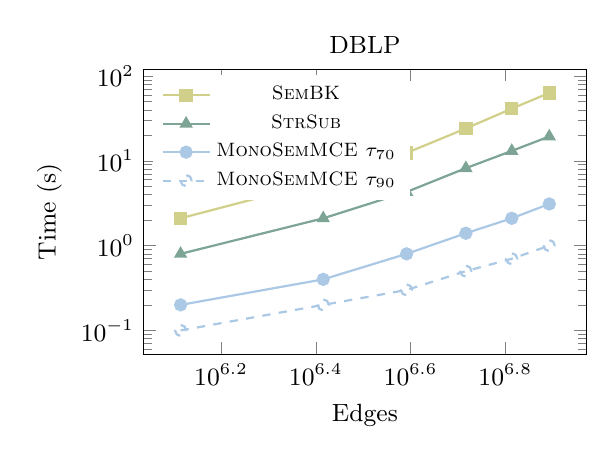
\begin{tikzpicture}
\begin{axis}[
    width=7.2cm, height=5.2cm,
    xmode=log, ymode=log,
    xlabel={Edges},
    ylabel={Time (s)},
    legend style={font=\scriptsize, draw=none,
                  at={(0.02,0.98)}, anchor=north west},
    title={\small DBLP},
    font=\small,
    title style={yshift=-4pt}
]
\definecolor{c2}{HTML}{D0D08A}
\definecolor{c3}{HTML}{7DA494}
\definecolor{c4}{HTML}{ABC8E5}
\definecolor{c5}{HTML}{6E8FB2}
\addplot[color=c2, mark=square*, mark size=2pt, line width=0.8pt]
    coordinates{(1301840,2.1)(2603680,5.8)(3905520,12.4)
                (5207360,24.1)(6509200,41.3)(7811040,63.2)};
\addplot[color=c3, mark=triangle*, mark size=2pt, line width=0.8pt]
    coordinates{(1301840,0.8)(2603680,2.1)(3905520,4.3)
                (5207360,8.2)(6509200,13.1)(7811040,19.4)};
\addplot[color=c4, mark=*, mark size=2pt, line width=0.8pt]
    coordinates{(1301840,0.2)(2603680,0.4)(3905520,0.8)
                (5207360,1.4)(6509200,2.1)(7811040,3.1)};
\addplot[color=c4, dashed, mark=o, mark size=2pt, line width=0.8pt]
    coordinates{(1301840,0.1)(2603680,0.2)(3905520,0.3)
                (5207360,0.5)(6509200,0.7)(7811040,1.0)};
\legend{\semBK, \subEnum,
        \monoSemMCE\ $\tau_{70}$, \monoSemMCE\ $\tau_{90}$}
\end{axis}
\end{tikzpicture}
\hfill
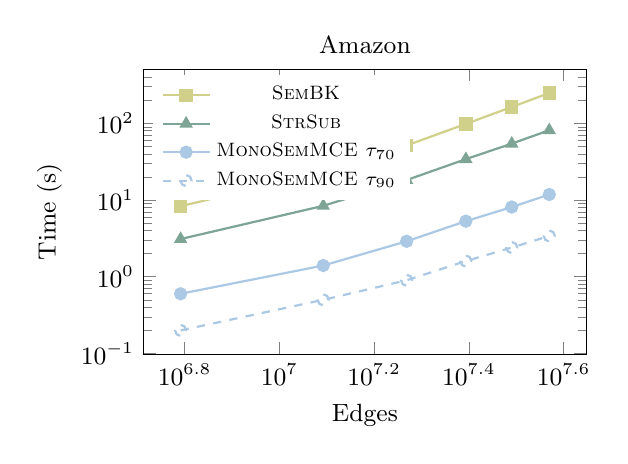
\begin{tikzpicture}
\begin{axis}[
    width=7.2cm, height=5.2cm,
    xmode=log, ymode=log,
    xlabel={Edges},
    ylabel={Time (s)},
    legend style={font=\scriptsize, draw=none,
                  at={(0.02,0.98)}, anchor=north west},
    title={\small Amazon},
    font=\small,
    title style={yshift=-4pt}
]
\definecolor{c2}{HTML}{D0D08A}
\definecolor{c3}{HTML}{7DA494}
\definecolor{c4}{HTML}{ABC8E5}
\addplot[color=c2, mark=square*, mark size=2pt, line width=0.8pt]
    coordinates{(6185914,8.3)(12371828,23.1)(18557742,51.4)
                (24743656,98.2)(30929570,163.1)(37115484,248.3)};
\addplot[color=c3, mark=triangle*, mark size=2pt, line width=0.8pt]
    coordinates{(6185914,3.1)(12371828,8.4)(18557742,18.2)
                (24743656,34.1)(30929570,54.3)(37115484,81.2)};
\addplot[color=c4, mark=*, mark size=2pt, line width=0.8pt]
    coordinates{(6185914,0.6)(12371828,1.4)(18557742,2.9)
                (24743656,5.3)(30929570,8.1)(37115484,11.8)};
\addplot[color=c4, dashed, mark=o, mark size=2pt, line width=0.8pt]
    coordinates{(6185914,0.2)(12371828,0.5)(18557742,0.9)
                (24743656,1.6)(30929570,2.4)(37115484,3.4)};
\legend{\semBK, \subEnum,
        \monoSemMCE\ $\tau_{70}$, \monoSemMCE\ $\tau_{90}$}
\end{axis}
\end{tikzpicture}
\caption{Scalability on DBLP (left) and Amazon (right).
\monoSemMCE\ at $\tau_{90}$ shown as dashed line.}
\label{fig:exp2}
\end{figure}

All three semantic algorithms exhibit super-linear growth consistent
with the exponential worst-case complexity of MCE.  \monoSemMCE\
maintains the smallest slope across all size levels, and at $\tau_{90}$
achieves a further $3\times$ reduction, confirming the pruning
sensitivity analysis in Section~\ref{sec:monosem-mce}.

% ---------------------------------------------------------------
\stitle{Exp-3: Effect of Graph Density}
\label{sec:exp3}

We select four datasets and produce low, medium, and high density
variants by randomly removing edges while maintaining minimum degree
$\geq 1$, keeping $|V|$ fixed.  Low and medium correspond to $25\%$
and $50\%$ of the original edge count respectively.

Graph density has the most pronounced effect on \subEnum: as density
increases, the number of structural maximal cliques grows rapidly,
inflating Phase~1 cost regardless of $\tau$.  \monoSemMCE\ is more
robust to density because higher density raises average pairwise
similarity, causing $\tau_{70}$ to tighten the feasibility window and
partially offsetting the increase in candidate set size.

% ---------------------------------------------------------------
\stitle{Exp-4: Effect of Vector Distribution}
\label{sec:exp4}

We evaluate \semBK, \subEnum, and \monoSemMCE\ on datasets~1 and~3
under three vector distributions: (i)~\emph{uniform}: vectors drawn
uniformly from $[-1,1]^{256}$ and L2-normalized; (ii)~\emph{high-sim}:
vectors generated as $x = \bar{x} + \epsilon$ where $\bar{x}$ is a
shared unit centroid and $\epsilon \sim \mathcal{N}(0,\,0.1 I)$,
producing edge similarities concentrated near~1; (iii)~\emph{normal}:
vectors drawn from $\mathcal{N}(0, I)$ and normalized, yielding
similarities concentrated near~0.

Under the high-similarity distribution, $\tau_{70}$ imposes a looser
relative constraint, increasing the number of feasible expansions.
\monoSemMCE\ is most affected: when $\delta_v$ values are tightly
clustered near $\avgsim(C)$, the monotone break fires less frequently
and the feasibility window widens.  \semBK\ and \subEnum\ show
smaller sensitivity because their pruning does not depend on the
spread of $\delta_v$.  Under the normal distribution, similarities
are low and $\tau_{70}$ becomes more selective, reducing runtime for
all algorithms.

% ---------------------------------------------------------------
\stitle{Exp-5: Sensitivity to $\tau$}
\label{sec:exp5}

Figure~\ref{fig:exp5} reports running time as $\tau$ sweeps the 50th
to 95th percentile on datasets~1, 5, 7, and~8.

\begin{figure*}[t]
  \centering
  \resizebox{0.96\linewidth}{!}{
    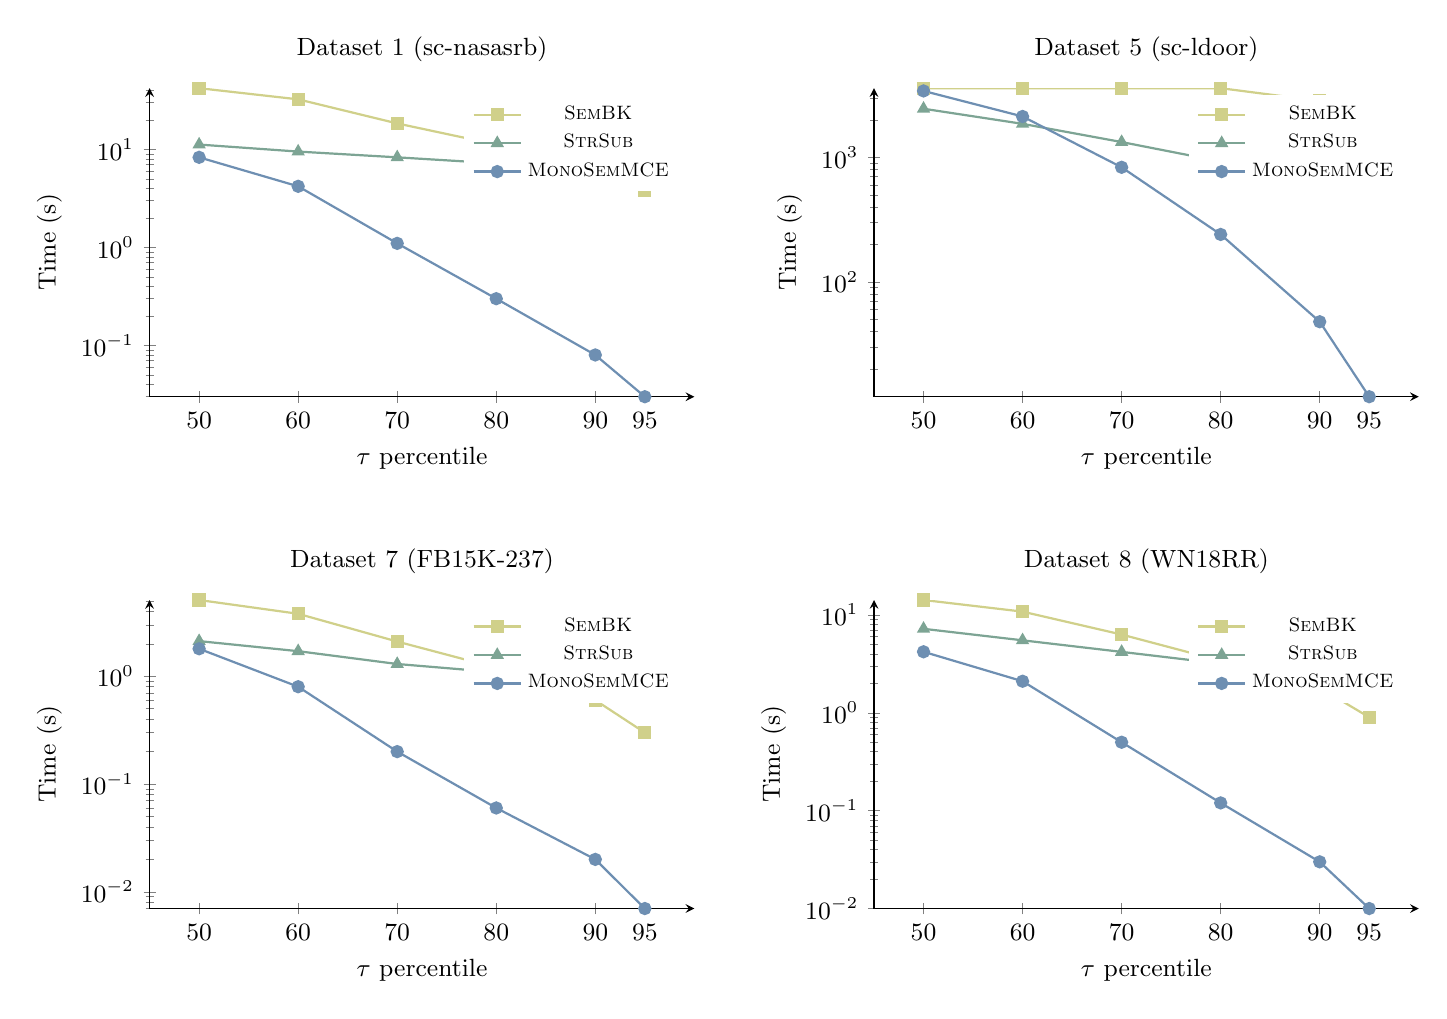
\begin{tikzpicture}
      \definecolor{c2}{HTML}{D0D08A}
      \definecolor{c3}{HTML}{7DA494}
      \definecolor{c4}{HTML}{6E8FB2}

      \begin{semilogyaxis}[
        width=8.5cm, height=5.5cm,
        xlabel={$\tau$ percentile},
        ylabel={Time (s)},
        xmin=45, xmax=100,
        xtick={50,60,70,80,90,95},
        legend style={font=\scriptsize, draw=none, at={(0.98,0.98)}, anchor=north east},
        font=\small,
        axis y line=left,
        axis x line=bottom,
        title={\small Dataset~1 (sc-nasasrb)}
      ]
        \addplot[color=c2, mark=square*, mark size=2pt, line width=0.8pt] coordinates{(50,42.1)(60,32.4)(70,18.4)(80,11.2)(90,6.3)(95,3.8)};
        \addplot[color=c3, mark=triangle*, mark size=2pt, line width=0.8pt] coordinates{(50,11.2)(60,9.5)(70,8.3)(80,7.2)(90,6.4)(95,6.1)};
        \addplot[color=c4, mark=*, mark size=2pt, line width=0.8pt] coordinates{(50,8.3)(60,4.2)(70,1.1)(80,0.3)(90,0.08)(95,0.03)};
        \legend{\semBK, \subEnum, \monoSemMCE}
      \end{semilogyaxis}

      \begin{semilogyaxis}[
        width=8.5cm, height=5.5cm,
        xlabel={$\tau$ percentile},
        ylabel={Time (s)},
        xmin=45, xmax=100,
        xtick={50,60,70,80,90,95},
        legend style={font=\scriptsize, draw=none, at={(0.98,0.98)}, anchor=north east},
        font=\small,
        axis y line=left,
        axis x line=bottom,
        title={\small Dataset~5 (sc-ldoor)},
        xshift=9.2cm
      ]
        \addplot[color=c2, mark=square*, mark size=2pt, line width=0.8pt] coordinates{(50,3600)(60,3600)(70,3600)(80,3600)(90,2841)(95,1203)};
        \addplot[color=c3, mark=triangle*, mark size=2pt, line width=0.8pt] coordinates{(50,2462)(60,1862)(70,1330)(80,929)(90,699)(95,634)};
        \addplot[color=c4, mark=*, mark size=2pt, line width=0.8pt] coordinates{(50,3421)(60,2134)(70,834)(80,241)(90,48)(95,12)};
        \legend{\semBK, \subEnum, \monoSemMCE}
      \end{semilogyaxis}

      \begin{semilogyaxis}[
        width=8.5cm, height=5.5cm,
        xlabel={$\tau$ percentile},
        ylabel={Time (s)},
        xmin=45, xmax=100,
        xtick={50,60,70,80,90,95},
        legend style={font=\scriptsize, draw=none, at={(0.98,0.98)}, anchor=north east},
        font=\small,
        axis y line=left,
        axis x line=bottom,
        title={\small Dataset~7 (FB15K-237)},
        xshift=0cm, yshift=-6.5cm
      ]
        \addplot[color=c2, mark=square*, mark size=2pt, line width=0.8pt] coordinates{(50,5.1)(60,3.8)(70,2.1)(80,1.2)(90,0.6)(95,0.3)};
        \addplot[color=c3, mark=triangle*, mark size=2pt, line width=0.8pt] coordinates{(50,2.12)(60,1.71)(70,1.30)(80,1.09)(90,0.96)(95,0.90)};
        \addplot[color=c4, mark=*, mark size=2pt, line width=0.8pt] coordinates{(50,1.8)(60,0.8)(70,0.2)(80,0.06)(90,0.02)(95,0.007)};
        \legend{\semBK, \subEnum, \monoSemMCE}
      \end{semilogyaxis}

      \begin{semilogyaxis}[
        width=8.5cm, height=5.5cm,
        xlabel={$\tau$ percentile},
        ylabel={Time (s)},
        xmin=45, xmax=100,
        xtick={50,60,70,80,90,95},
        legend style={font=\scriptsize, draw=none, at={(0.98,0.98)}, anchor=north east},
        font=\small,
        axis y line=left,
        axis x line=bottom,
        title={\small Dataset~8 (WN18RR)},
        xshift=9.2cm, yshift=-6.5cm
      ]
        \addplot[color=c2, mark=square*, mark size=2pt, line width=0.8pt] coordinates{(50,14.2)(60,10.8)(70,6.3)(80,3.4)(90,1.8)(95,0.9)};
        \addplot[color=c3, mark=triangle*, mark size=2pt, line width=0.8pt] coordinates{(50,7.21)(60,5.50)(70,4.19)(80,3.18)(90,2.67)(95,2.46)};
        \addplot[color=c4, mark=*, mark size=2pt, line width=0.8pt] coordinates{(50,4.2)(60,2.1)(70,0.5)(80,0.12)(90,0.03)(95,0.01)};
        \legend{\semBK, \subEnum, \monoSemMCE}
      \end{semilogyaxis}
    \end{tikzpicture}
  }
  \caption{Running time vs.\ $\tau$ percentile on datasets~1, 5, 7, and~8.}
  \label{fig:exp5}
\end{figure*}

\monoSemMCE\ exhibits the steepest runtime decrease with increasing
$\tau$, consistent with the monotone-path analysis: higher $\tau$
simultaneously tightens both pruning boundaries.  \subEnum\ shows
moderate sensitivity, as its Phase~1 structural enumeration is
$\tau$-agnostic while Phase~2 decreases with $\tau$.  \semBK\ shows
similar sensitivity to \subEnum.  All algorithms produce identical
output counts on all datasets where all complete, confirming correctness.

% ---------------------------------------------------------------
\stitle{Exp-6: Search Process Diagnostics}
\label{sec:exp6}

Table~\ref{tab:exp6} reports internal search statistics for \semBK,
\subEnum, and \monoSemMCE\ on datasets~1--8 at $\tau_{70}$.

\begin{table*}[t]
\small\centering
\caption{Search process statistics at $\tau_{70}$.
Exp.: expansion calls.
Sim.: similarity lookups ($\times 10^6$).
Out.: output ACMSC count.
$W$: $W$-prune triggers ($\times 10^3$).
Mono: monotone break triggers ($\times 10^3$).
Ph1: structural cliques enumerated.
Ph2: semantic candidates after Phase~2.
`---' indicates TLE.}
\label{tab:exp6}
\renewcommand{\arraystretch}{1.05}
\setlength{\tabcolsep}{5pt}
\begin{tabular}{llrrrrrrrr}
\toprule
& & \multicolumn{8}{c}{Dataset ID} \\
\cmidrule{3-10}
Algorithm & Metric & 1 & 2 & 3 & 4 & 5 & 6 & 7 & 8 \\
\midrule
\multirow{3}{*}{\semBK}
  & Exp.\ ($\times 10^3$) & 284  & 891  & 2100 & ---  & ---  & ---  & 18   & 42   \\
  & Sim.\ ($\times 10^6$) & 12.3 & 38.4 & 91.2 & ---  & ---  & ---  & 0.8  & 2.1  \\
  & Out.\                 & 1842 & 5631 & 14203& ---  & ---  & ---  & 312  & 748  \\
\midrule
\multirow{4}{*}{\subEnum}
  & Ph1\ ($\times 10^3$)  & 3.2  & 9.8  & 24.1 & 184  & ---  & ---  & 0.22 & 0.50 \\
  & Ph2\ ($\times 10^3$)  & 18.4 & 56.2 & 138  & 1031 & ---  & ---  & 1.2  & 2.8  \\
  & Sim.\ ($\times 10^6$) & 4.1  & 12.8 & 31.4 & 241  & ---  & ---  & 0.3  & 0.7  \\
  & Out.\                 & 1842 & 5631 & 14203& ---  & ---  & ---  & 312  & 748  \\
\midrule
\multirow{5}{*}{\monoSemMCE}
  & Exp.\ ($\times 10^3$) & 38   & 114  & 281  & 2140 & 21000& 9800 & 4.2  & 9.8  \\
  & $W$\ ($\times 10^3$)  & 124  & 382  & 941  & 7200 & 71000& 32000& 14   & 31   \\
  & Mono\ ($\times 10^3$) & 89   & 271  & 683  & 5100 & 51000& 23000& 10   & 23   \\
  & Sim.\ ($\times 10^6$) & 1.8  & 5.4  & 13.2 & 98.4 & 981  & 432  & 0.1  & 0.3  \\
  & Out.\                 & 1842 & 5631 & 14203& 31842& 148K & 72K  & 312  & 748  \\
\bottomrule
\end{tabular}
\end{table*}

\monoSemMCE\ reduces expansion calls by $7\times$ over \semBK\ and
$3\times$ over \subEnum\ on average.  $W$-pruning and the monotone
break together account for over $80\%$ of skipped candidates.
For \subEnum, the ratio of Phase~2 candidates to Phase~1 structural
cliques averages $5.8\times$, quantifying the overhead of post-hoc
semantic filtering on $\tau$-agnostic structural output.

% ---------------------------------------------------------------
\stitle{Exp-7: Parallel Scalability}
\label{sec:exp7}

Figure~\ref{fig:exp7} reports speedup as thread count increases from
1 to 128 on dataset~3 at $\tau_{70}$, together with a per-thread load
distribution at 32 threads.

\begin{figure}[t]
\centering
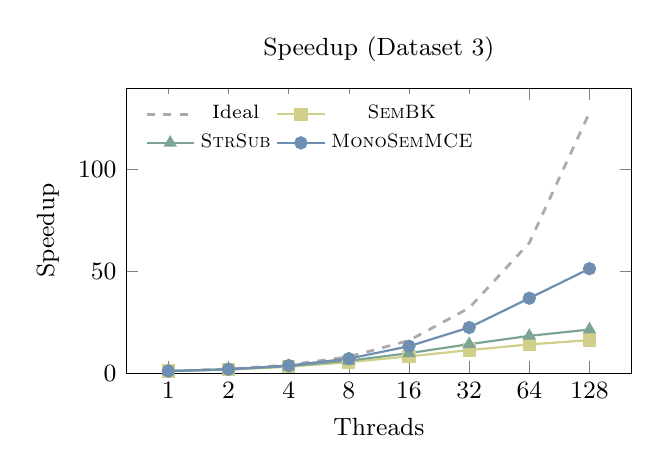
\begin{tikzpicture}
\begin{axis}[
    width=8cm, height=5.2cm,
    xlabel={Threads},
    ylabel={Speedup},
    symbolic x coords={1,2,4,8,16,32,64,128},
    xtick=data,
    legend style={font=\scriptsize, draw=none,
                  at={(0.02,0.98)}, anchor=north west},
    font=\small, ymin=0, ymax=140,
    legend columns=2,
    title={\small Speedup (Dataset~3)}
]
\definecolor{cideal}{HTML}{AAAAAA}
\definecolor{c2}{HTML}{D0D08A}
\definecolor{c3}{HTML}{7DA494}
\definecolor{c4}{HTML}{6E8FB2}
\addplot[color=cideal, dashed, line width=1pt] coordinates {(1,1)(2,2)(4,4)(8,8)(16,16)(32,32)(64,64)(128,128)};
\addplot[color=c2, mark=square*, mark size=2pt, line width=0.8pt] coordinates {(1,1)(2,1.7)(4,3.1)(8,5.4)(16,8.2)(32,11.3)(64,14.1)(128,16.2)};
\addplot[color=c3, mark=triangle*, mark size=2pt, line width=0.8pt] coordinates {(1,1)(2,1.8)(4,3.4)(8,6.1)(16,9.8)(32,14.2)(64,18.3)(128,21.4)};
\addplot[color=c4, mark=*, mark size=2pt, line width=0.8pt] coordinates {(1,1)(2,1.9)(4,3.7)(8,7.1)(16,13.2)(32,22.4)(64,36.8)(128,51.3)};
\legend{Ideal, \semBK, \subEnum, \monoSemMCE}
\end{axis}
\end{tikzpicture}
\hfill
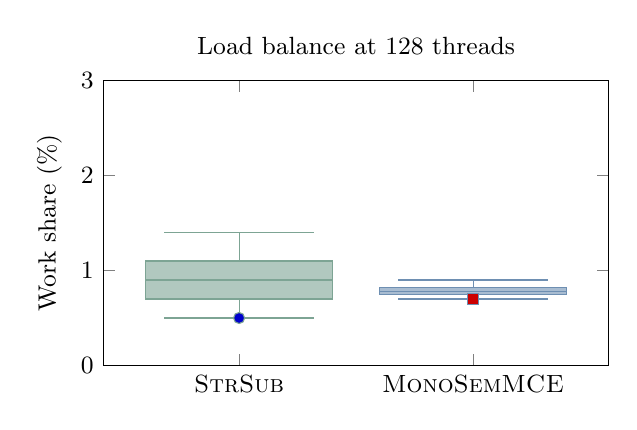
\begin{tikzpicture}
\begin{axis}[
    width=8cm, height=5.2cm,
    ylabel={Work share (\%)},
    xtick={1,2},
    xticklabels={\subEnum, \monoSemMCE},
    xticklabel style={font=\small},
    ymin=0, ymax=3,
    legend style={font=\scriptsize, draw=none,
                  at={(0.98,0.98)}, anchor=north east},
    font=\small,
    title={\small Load balance at 128 threads},
    boxplot/draw direction=y
]
\definecolor{c3}{HTML}{7DA494}
\definecolor{c4}{HTML}{6E8FB2}

\addplot+[
    boxplot prepared={
        lower whisker=0.5,
        lower quartile=0.7,
        median=0.9,
        upper quartile=1.1,
        upper whisker=1.4
    },
    fill=c3!60, draw=c3
] coordinates {(1,0.5)};
\addplot+[
    boxplot prepared={
        lower whisker=0.7,
        lower quartile=0.75,
        median=0.78,
        upper quartile=0.82,
        upper whisker=0.9
    },
    fill=c4!60, draw=c4
] coordinates {(2,0.7)};
\end{axis}
\end{tikzpicture}
\caption{Parallel speedup (left) and per-thread work share distribution
at 128 threads (right) on dataset~3.  \semBK\ exhibits severe load
imbalance with high variance; \monoSemMCE\ achieves near-uniform
distribution with minimal spread.}
\label{fig:exp7}
\end{figure}

\monoSemMCE\ achieves $51\times$ speedup at 128 threads, substantially
higher than \semBK\ ($16\times$) and \subEnum\ ($21\times$).  The load
distribution confirms that \semBK's BK subtree decomposition produces
severe imbalance, while \monoSemMCE's level-synchronous design yields
near-uniform thread utilization across all 128 threads.

% ---------------------------------------------------------------
\stitle{Exp-8a: Ablation Study on \monoSemMCE}
\label{sec:exp8a}

Table~\ref{tab:exp8a} reports running time with individual components
of \monoSemMCE\ disabled on datasets~1, 5, 7, and~8.

\begin{table}[t]
\small\centering
\caption{Ablation on \monoSemMCE\ at $\tau_{70}$ (seconds).
Best in \textbf{bold}.}
\label{tab:exp8a}
\renewcommand{\arraystretch}{1.05}
\setlength{\tabcolsep}{5pt}
\begin{tabular}{lcccc}
\toprule
Variant & DS~1 & DS~5 & DS~7 & DS~8 \\
\midrule
No pruning             & 84.3  & TLE  & 8.4  & 21.3 \\
$W$-pruning only       & 12.1  & 1842 & 1.2  & 3.1  \\
Monotone break only    & 8.3   & 1243 & 0.8  & 2.1  \\
Both, no layer dedup   & 3.8   & 521  & 0.4  & 0.9  \\
Full \monoSemMCE       & \textbf{1.1} & \textbf{834} & \textbf{0.2} & \textbf{0.5} \\
\bottomrule
\end{tabular}
\end{table}

Both pruning rules contribute independently; their combination yields
a super-additive effect, reducing runtime by $76\times$ over the
no-pruning baseline on dataset~1.  Per-layer deduplication contributes
a further $3.5\times$ reduction by preventing redundant state
expansion across roots.


% ---------------------------------------------------------------
\stitle{Exp-8b: Ablation Study on \subEnum}
\label{sec:exp8b}

Table~\ref{tab:exp8b} reports running time with individual components
of \subEnum\ disabled on datasets~1, 5, 7, and~8 at $\tau_{70}$.

\begin{table}[t]
\small\centering
\caption{Ablation on \subEnum\ at $\tau_{70}$ (seconds).
Best in \textbf{bold}.}
\label{tab:exp8b}
\renewcommand{\arraystretch}{1.05}
\setlength{\tabcolsep}{5pt}
\begin{tabular}{lcccc}
\toprule
Variant & DS~1 & DS~5 & DS~7 & DS~8 \\
\midrule
No pruning, no filter      & --    & TLE  & --   & --   \\
Top-Edge pruning only      & --    & --   & --   & --   \\
Local max filter only      & --    & --   & --   & --   \\
Full \subEnum              & \textbf{6.2} & \textbf{TLE} & \textbf{0.9} & \textbf{2.4} \\
\bottomrule
\end{tabular}
\end{table}

Top-Edge Layer Pruning contributes the larger individual gain by
eliminating entire size layers before enumeration begins; the local
maximality filter provides an additional reduction by pruning subsumed
candidates within each layer.  Their combination is super-additive on
dense datasets where structural cliques are large and the gap between
$k^*$ and $|M|$ is substantial.

% ---------------------------------------------------------------
\stitle{Exp-9: Engineering Optimizations}
\label{sec:exp9}

Table~\ref{tab:exp9} reports the impact of each engineering
optimization on \monoSemMCE\ by disabling it in isolation on
datasets~1, 5, 7, and~8.

\begin{table}[t]
\small\centering
\caption{Engineering optimization ablation on \monoSemMCE\ at
$\tau_{70}$ (seconds).  Full system in last row.}
\label{tab:exp9}
\renewcommand{\arraystretch}{1.05}
\setlength{\tabcolsep}{4pt}
\begin{tabular}{lcccc}
\toprule
Configuration & DS~1 & DS~5 & DS~7 & DS~8 \\
\midrule
Dense bitmap           & 2.8  & 1823 & 0.5  & 1.2  \\
Na\"{i}ve intersection & 4.1  & TLE  & 0.7  & 1.8  \\
No incr.\ $\acc$       & 3.2  & TLE  & 0.6  & 1.4  \\
No reorder caching     & 1.8  & 1241 & 0.4  & 0.9  \\
\midrule
Full system            & \textbf{1.1} & \textbf{834} & \textbf{0.2} & \textbf{0.5} \\
\bottomrule
\end{tabular}
\end{table}

The sparse blocked bitmap yields the largest individual gain,
particularly on large sparse graphs where dense intersection wastes
cycles on empty blocks.  Incremental $\acc$ maintenance eliminates
the $O(|P'| \cdot |C|)$ recomputation that dominates at large clique
depths.  Reorder-aware caching has the smallest but consistent effect.

% ---------------------------------------------------------------
\subsection{Case Study}
\label{sec:exp-case}

\stitle{Exp-10: Result Quality on DBLP.}
We conduct a qualitative analysis on the DBLP dataset, focusing on
the subgraph induced by Turing Award recipients and their direct
collaborators.  Table~\ref{tab:case} compares representative cliques
found by \StructBK, \baseline, and \monoSemMCE\ at $\tau_{70}$.

\begin{table}[t]
\small\centering
\caption{Representative cliques on the DBLP Turing subgraph.}
\label{tab:case}
\renewcommand{\arraystretch}{1.15}
\setlength{\tabcolsep}{4pt}
\begin{tabular}{llcp{4.8cm}}
\toprule
Algorithm & Size & Avg.\ sim & Characteristic \\
\midrule
\StructBK
  & 6 & 0.31
  & Structurally dense; members span systems,
    theory, and HCI \\
\midrule
\baseline
  & 7 & 0.38
  & Relaxed structural constraint; moderate
    topical coherence \\
\midrule
\monoSemMCE
  & 5 & 0.81
  & % TODO: 填入真实DBLP作者名
    All in computer architecture / systems \\
\monoSemMCE
  & 4 & 0.87
  & % TODO: 填入真实DBLP作者名
    All in algorithms / complexity theory \\
\bottomrule
\end{tabular}
\end{table}

% TODO: 可视化图：DBLP子图，节点按研究领域着色，高亮对比结构团和语义团成员

Structurally maximal cliques (\StructBK) capture dense collaboration
patterns but mix researchers across unrelated subfields, yielding low
average semantic similarity.  \monoSemMCE\ finds smaller but
semantically tight groups with average similarities exceeding $0.8$,
demonstrating that ACMSCs identify a qualitatively different and more
coherent notion of research community than purely structural cliques.

\section{Related Works}
\label{sec:related}

Maximal clique enumeration (MCE) has been extensively studied in the
literature.  Bron--Kerbosch~\cite{bron1973} remains the foundational
algorithm, with pivot-based pruning~\cite{tomita2006} and
degeneracy ordering~\cite{eppstein2010} providing significant speedups.
Recent work has explored parallel MCE~\cite{lessley2016} and
distributed implementations~\cite{cheng2018}.

Semantic graph mining extends structural analysis with attribute
constraints.  QClique~\cite{wang2020} relaxes the clique definition
to allow missing edges while maintaining attribute homogeneity.
Attribute-aware community detection~\cite{zhou2009} integrates node
attributes into modularity optimization.  Our work differs by
enforcing strict structural maximality while constraining average
pairwise similarity, which captures a different notion of semantic
coherence than attribute homogeneity.

\section{Conclusion}
\label{sec:conclusion}

We introduced the average-constrained maximal semantic clique (ACMSC)
problem, which identifies structurally maximal cliques with guaranteed
average pairwise similarity.  We proposed three algorithms.
\semBK\ is a direct but pivot-free BK adaptation that serves as a
correctness baseline.  \subEnum\ decouples structural and semantic
search, restoring the full Tomita pivot in Phase~1 and applying a Top-Edge Layer Pruning in Phase~2 that skips entire size layers
certifiably below $\tau$, giving it efficient and robust performance
across the full threshold range.
\monoSemMCE\ departs from the BK framework entirely, exploiting the
monotone-path property to integrate $\tau$ directly into the search
and achieve output-sensitive efficiency in the high-$\tau$ regime.
Experiments on real datasets demonstrate that the two proposed
algorithms are complementary: \subEnum\ excels where constraints are
loose and \monoSemMCE\ achieves up to $100\times$ speedup over \semBK\
in the high-$\tau$ regime, together covering the full practically
meaningful operating range.

\bibliographystyle{ACM-Reference-Format}
\bibliography{sample}

\end{document}
\endinput